% Options for packages loaded elsewhere
% Options for packages loaded elsewhere
\PassOptionsToPackage{unicode}{hyperref}
\PassOptionsToPackage{hyphens}{url}
\PassOptionsToPackage{dvipsnames,svgnames,x11names}{xcolor}
%
\documentclass[
  letterpaper,
  DIV=11,
  numbers=noendperiod,
  oneside]{scrartcl}
\usepackage{xcolor}
\usepackage[left=1in,marginparwidth=2.0666666666667in,textwidth=4.1333333333333in,marginparsep=0.3in]{geometry}
\usepackage{amsmath,amssymb}
\setcounter{secnumdepth}{5}
\usepackage{iftex}
\ifPDFTeX
  \usepackage[T1]{fontenc}
  \usepackage[utf8]{inputenc}
  \usepackage{textcomp} % provide euro and other symbols
\else % if luatex or xetex
  \usepackage{unicode-math} % this also loads fontspec
  \defaultfontfeatures{Scale=MatchLowercase}
  \defaultfontfeatures[\rmfamily]{Ligatures=TeX,Scale=1}
\fi
\usepackage{lmodern}
\ifPDFTeX\else
  % xetex/luatex font selection
\fi
% Use upquote if available, for straight quotes in verbatim environments
\IfFileExists{upquote.sty}{\usepackage{upquote}}{}
\IfFileExists{microtype.sty}{% use microtype if available
  \usepackage[]{microtype}
  \UseMicrotypeSet[protrusion]{basicmath} % disable protrusion for tt fonts
}{}
\makeatletter
\@ifundefined{KOMAClassName}{% if non-KOMA class
  \IfFileExists{parskip.sty}{%
    \usepackage{parskip}
  }{% else
    \setlength{\parindent}{0pt}
    \setlength{\parskip}{6pt plus 2pt minus 1pt}}
}{% if KOMA class
  \KOMAoptions{parskip=half}}
\makeatother
% Make \paragraph and \subparagraph free-standing
\makeatletter
\ifx\paragraph\undefined\else
  \let\oldparagraph\paragraph
  \renewcommand{\paragraph}{
    \@ifstar
      \xxxParagraphStar
      \xxxParagraphNoStar
  }
  \newcommand{\xxxParagraphStar}[1]{\oldparagraph*{#1}\mbox{}}
  \newcommand{\xxxParagraphNoStar}[1]{\oldparagraph{#1}\mbox{}}
\fi
\ifx\subparagraph\undefined\else
  \let\oldsubparagraph\subparagraph
  \renewcommand{\subparagraph}{
    \@ifstar
      \xxxSubParagraphStar
      \xxxSubParagraphNoStar
  }
  \newcommand{\xxxSubParagraphStar}[1]{\oldsubparagraph*{#1}\mbox{}}
  \newcommand{\xxxSubParagraphNoStar}[1]{\oldsubparagraph{#1}\mbox{}}
\fi
\makeatother


\usepackage{longtable,booktabs,array}
\usepackage{calc} % for calculating minipage widths
% Correct order of tables after \paragraph or \subparagraph
\usepackage{etoolbox}
\makeatletter
\patchcmd\longtable{\par}{\if@noskipsec\mbox{}\fi\par}{}{}
\makeatother
% Allow footnotes in longtable head/foot
\IfFileExists{footnotehyper.sty}{\usepackage{footnotehyper}}{\usepackage{footnote}}
\makesavenoteenv{longtable}
\usepackage{graphicx}
\makeatletter
\newsavebox\pandoc@box
\newcommand*\pandocbounded[1]{% scales image to fit in text height/width
  \sbox\pandoc@box{#1}%
  \Gscale@div\@tempa{\textheight}{\dimexpr\ht\pandoc@box+\dp\pandoc@box\relax}%
  \Gscale@div\@tempb{\linewidth}{\wd\pandoc@box}%
  \ifdim\@tempb\p@<\@tempa\p@\let\@tempa\@tempb\fi% select the smaller of both
  \ifdim\@tempa\p@<\p@\scalebox{\@tempa}{\usebox\pandoc@box}%
  \else\usebox{\pandoc@box}%
  \fi%
}
% Set default figure placement to htbp
\def\fps@figure{htbp}
\makeatother


% definitions for citeproc citations
\NewDocumentCommand\citeproctext{}{}
\NewDocumentCommand\citeproc{mm}{%
  \begingroup\def\citeproctext{#2}\cite{#1}\endgroup}
\makeatletter
 % allow citations to break across lines
 \let\@cite@ofmt\@firstofone
 % avoid brackets around text for \cite:
 \def\@biblabel#1{}
 \def\@cite#1#2{{#1\if@tempswa , #2\fi}}
\makeatother
\newlength{\cslhangindent}
\setlength{\cslhangindent}{1.5em}
\newlength{\csllabelwidth}
\setlength{\csllabelwidth}{3em}
\newenvironment{CSLReferences}[2] % #1 hanging-indent, #2 entry-spacing
 {\begin{list}{}{%
  \setlength{\itemindent}{0pt}
  \setlength{\leftmargin}{0pt}
  \setlength{\parsep}{0pt}
  % turn on hanging indent if param 1 is 1
  \ifodd #1
   \setlength{\leftmargin}{\cslhangindent}
   \setlength{\itemindent}{-1\cslhangindent}
  \fi
  % set entry spacing
  \setlength{\itemsep}{#2\baselineskip}}}
 {\end{list}}
\usepackage{calc}
\newcommand{\CSLBlock}[1]{\hfill\break\parbox[t]{\linewidth}{\strut\ignorespaces#1\strut}}
\newcommand{\CSLLeftMargin}[1]{\parbox[t]{\csllabelwidth}{\strut#1\strut}}
\newcommand{\CSLRightInline}[1]{\parbox[t]{\linewidth - \csllabelwidth}{\strut#1\strut}}
\newcommand{\CSLIndent}[1]{\hspace{\cslhangindent}#1}



\setlength{\emergencystretch}{3em} % prevent overfull lines

\providecommand{\tightlist}{%
  \setlength{\itemsep}{0pt}\setlength{\parskip}{0pt}}



 


%\usepackage{bm}
\usepackage{tikz}
\usepackage{iftex}
\ifLuaTeX
  \usepackage{luatex85}
\fi
\usepackage[all,2cell]{xy}
\UseAllTwocells
\usepackage{sectsty}
\usepackage{sidenotes}
\renewcommand{\marginnote}[2][]{\sidenotetext[#1]{\parbox{\marginparwidth}{#2}}}
%\renewcommand{\marginnote}[2][]{\@sidenotes@placemarginal{0}{\textsuperscript{1}~#2}}
\usepackage{enumitem}
\setlist[description]{style=multiline,leftmargin=5cm,itemsep=20pt}
\usepackage{xcolor}
\sectionfont{\color{red}\sectionrule{0pt}{0pt}{-4pt}{1pt}}
\subsectionfont{\color{red}\sectionrule{0pt}{0pt}{-4pt}{.1pt}}
\newcommand{\ut}[2]{\underbrace{#1}_{\text{#2}}}
\newcommand{\utt}[3]{\underbrace{#1}_{\substack{\text{#2}\\\text{#3}}}}
\newcommand{\bm}[1]{\boldsymbol{#1}}
\makeatletter
\renewcommand{\@maketitle}{
  \begin{center}
    {\LARGE\@title\par}
    \vskip 1em
    {\large\@author\hspace{1em}|\hspace{1em}\@date\par}
  \end{center}
}
\makeatother
\KOMAoption{captions}{tableheading}
\makeatletter
\@ifpackageloaded{caption}{}{\usepackage{caption}}
\AtBeginDocument{%
\ifdefined\contentsname
  \renewcommand*\contentsname{Table of contents}
\else
  \newcommand\contentsname{Table of contents}
\fi
\ifdefined\listfigurename
  \renewcommand*\listfigurename{List of Figures}
\else
  \newcommand\listfigurename{List of Figures}
\fi
\ifdefined\listtablename
  \renewcommand*\listtablename{List of Tables}
\else
  \newcommand\listtablename{List of Tables}
\fi
\ifdefined\figurename
  \renewcommand*\figurename{Figure}
\else
  \newcommand\figurename{Figure}
\fi
\ifdefined\tablename
  \renewcommand*\tablename{Table}
\else
  \newcommand\tablename{Table}
\fi
}
\@ifpackageloaded{float}{}{\usepackage{float}}
\floatstyle{ruled}
\@ifundefined{c@chapter}{\newfloat{codelisting}{h}{lop}}{\newfloat{codelisting}{h}{lop}[chapter]}
\floatname{codelisting}{Listing}
\newcommand*\listoflistings{\listof{codelisting}{List of Listings}}
\makeatother
\makeatletter
\makeatother
\makeatletter
\@ifpackageloaded{caption}{}{\usepackage{caption}}
\@ifpackageloaded{subcaption}{}{\usepackage{subcaption}}
\makeatother
\makeatletter
\@ifpackageloaded{sidenotes}{}{\usepackage{sidenotes}}
\@ifpackageloaded{marginnote}{}{\usepackage{marginnote}}
\makeatother
\usepackage{bookmark}
\IfFileExists{xurl.sty}{\usepackage{xurl}}{} % add URL line breaks if available
\urlstyle{same}
\hypersetup{
  pdftitle={Stylized Facts about AI \& Human Capabilities},
  pdfauthor={Tom Cunningham \& Ali Merali},
  colorlinks=true,
  linkcolor={blue},
  filecolor={Maroon},
  citecolor={Blue},
  urlcolor={Blue},
  pdfcreator={LaTeX via pandoc}}


\title{Stylized Facts about AI \& Human Capabilities}
\author{Tom Cunningham \& Ali Merali}
\date{2026-09-03}
\begin{document}
\maketitle
\begin{abstract}
We discuss stylized facts about the capabilities of recent AI models and
how they compare to human capabilities. We particularly draw attention
to a common latent factor of capabilities among AI models, and the fact
that this latent factor is different from the distribution of human
capabilities. We discuss various candidates for the ``missing
capability'' which would unlock a greater economic impact.
\end{abstract}

\renewcommand*\contentsname{Table of contents}
{
\hypersetup{linkcolor=}
\setcounter{tocdepth}{2}
\tableofcontents
}

\marginnote{\begin{footnotesize}

Thanks to many for their suggestions, especially those from the Economic
Research team at OpenAI, and Boaz Barak. The document includes
significant suggestions from OpenAI staff (Pamela Mishkin, Zoe Hitzig,
Gawesha Weeratunga, Ronnie Chatterji), and external academics: Catherine
Tucker, David Deming, Erik Brynjolfsson, Anton Korinek, Pascual
Restrepo.

\end{footnotesize}}

\section{Overview}\label{overview}

\subsection{We wish to characterize AI
capabilities}\label{we-wish-to-characterize-ai-capabilities}

\begin{description}
\item[Our goal is to give a crisp characterization of AI capabilities.]
We wish to answer questions like these:

\begin{enumerate}
\def\labelenumi{\arabic{enumi}.}
\tightlist
\item
  What types of tasks can AI models do / cannot do?
\item
  How do abilities differ among different AI models?
\item
  How do AI abilities differ from human abilities?
\item
  What are reasonable expectations about future AI abilities?
\end{enumerate}
\item[A running theme will be that the characterization of AI
capabilities is \emph{difficult}.]
There is a long history of struggle in making accurate generalizations
about the capabilities of artificial intelligence. There is little
consensus on how to describe the abilities of contemporary models.

In this note we list a series of well-documented facts about AI
capabilities, and make some more opinionated generalizations. The target
audience is economists who are interested in modeling the effects of AI
on various situations.
\end{description}

\marginnote{\begin{footnotesize}

\pandocbounded{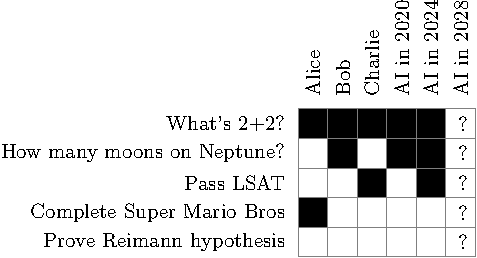
\includegraphics[keepaspectratio]{stylized-facts_files/figure-pdf/unnamed-chunk-1-1.pdf}}

\end{footnotesize}}

\begin{description}
\item[It is useful to think of a matrix of agents and tasks.]
Suppose we can observe whether an agent can perform a task, for a long
list of agents and tasks. The agent could be a human, a computer, or a
hybrid. We can represent each observation in a matrix with agents and
columns and tasks as rows:
\item[We wish to find a low-dimensional factorization of this matrix.]
In practice the matrix is enormous. We can think of the capability
problem as finding a low-dimensional representation of this matrix,
i.e.~some small set of general-purpose capabilities that are highly
predictive of whether an agent can do a task.\footnote{We can think of
  the reduction either as Principal Components Analysis (we take
  weighted averages of all rows), or Principal Feature Analysis (we take
  a subset of rows that are highly predictive).}

A single-dimensional factorization would mean each agent would have a
latent ability, and each task would have a latent difficulty. However we
will see that a single-factor is often a poor fit, i.e.~the relatively
difficulty of tasks varies substantially across agents.
\end{description}

\subsection{There is no standard measure of machine
intelligence}\label{there-is-no-standard-measure-of-machine-intelligence}

\begin{description}
\item[Many proposed measures of AGI have already been satisfied.]
Scott Alexander
\href{https://www.astralcodexten.com/p/sakana-strawberry-and-scary-ai}{says}
\emph{``The history of AI is people saying `We'll believe AI is Actually
Intelligent when it does X!' -- and then, after AI does X, not believing
it's Actually Intelligent.''}

Some examples:

\begin{longtable}[]{@{}
  >{\raggedright\arraybackslash}p{(\linewidth - 2\tabcolsep) * \real{0.8608}}
  >{\raggedright\arraybackslash}p{(\linewidth - 2\tabcolsep) * \real{0.1392}}@{}}
\toprule\noalign{}
\begin{minipage}[b]{\linewidth}\raggedright
Measure
\end{minipage} & \begin{minipage}[b]{\linewidth}\raggedright
Year passed
\end{minipage} \\
\midrule\noalign{}
\endhead
\bottomrule\noalign{}
\endlastfoot
Chess -- \emph{``Chess is generally considered to require `thinking' for
skilful play.''} --- Shannon, 1950. & 1997 \\
\href{https://en.wikipedia.org/wiki/Winograd_schema_challenge}{Winograd
Schemas} - \emph{``when people pass the test, we would say they were
thinking.''} & 2019 \\
\href{https://mmmu-benchmark.github.io/}{MMMU} -- \emph{``Benchmark for
Expert AGI.''} & 2025 \\
\href{https://github.com/fchollet/ARC-AGI}{ARC-AGI} -- \emph{``the only
formal benchmark of AGI progress.''} & 2024 \\
\href{https://github.com/ruixiangcui/AGIEval}{AGIEval} - \emph{``general
abilities \ldots{} in tasks pertinent to human cognition and
problem-solving.''} & 2025 \\
\end{longtable}
\item[There are some proposed definitions but none have become
canonical:]
\hfill
\begin{itemize}
\item
  Legg and Hutter (2007b) proposed ``intelligence measures an agent's
  ability to achieve goals in a wide range of environments.''\footnote{Additionally,
    Legg and Hutter (2007a) surveyed 70 different definitions of
    intelligence as of 2007.}
\item
  Chollet (2019) proposed intelligence be defined as ``skill-acquisition
  efficiency'', and proposed a formal benchmark (ARC-AGI).
\item
  Morris et al. (2023) proposed five ``levels of AGI'', based on the
  percentile human performance across all tasks. E.g. they classified
  ChatGPT as being able to do a \emph{``wide range of non-physical
  tasks, including metacognitive tasks like learning new skills equal to
  or somewhat better than an unskilled human.''}
\item
  In 2024 OpenAI internally developed a five-level scale of AGI, but it
  has not been publicly released.\footnote{https://www.bloomberg.com/news/articles/2024-07-11/openai-sets-levels-to-track-progress-toward-superintelligent-ai}
\item
  Hendrycks et al. (2025) proposed an AGI definition based on 10
  different sub-dimensions.
\end{itemize}
\end{description}

\subsection{There is no standard taxonomy of AI
capabilities.}\label{there-is-no-standard-taxonomy-of-ai-capabilities.}

\begin{description}
\tightlist
\item[There are hundreds of different AI benchmarks of capability.]
These benchmarks are often informally grouped into types which test
different types of ability, e.g.~``knowledge'', ``reasoning'',
``programming'', ``agentic ability'', however there is no
generally-accepted taxonomy.
\end{description}

\begin{figure}[H]

{\centering \pandocbounded{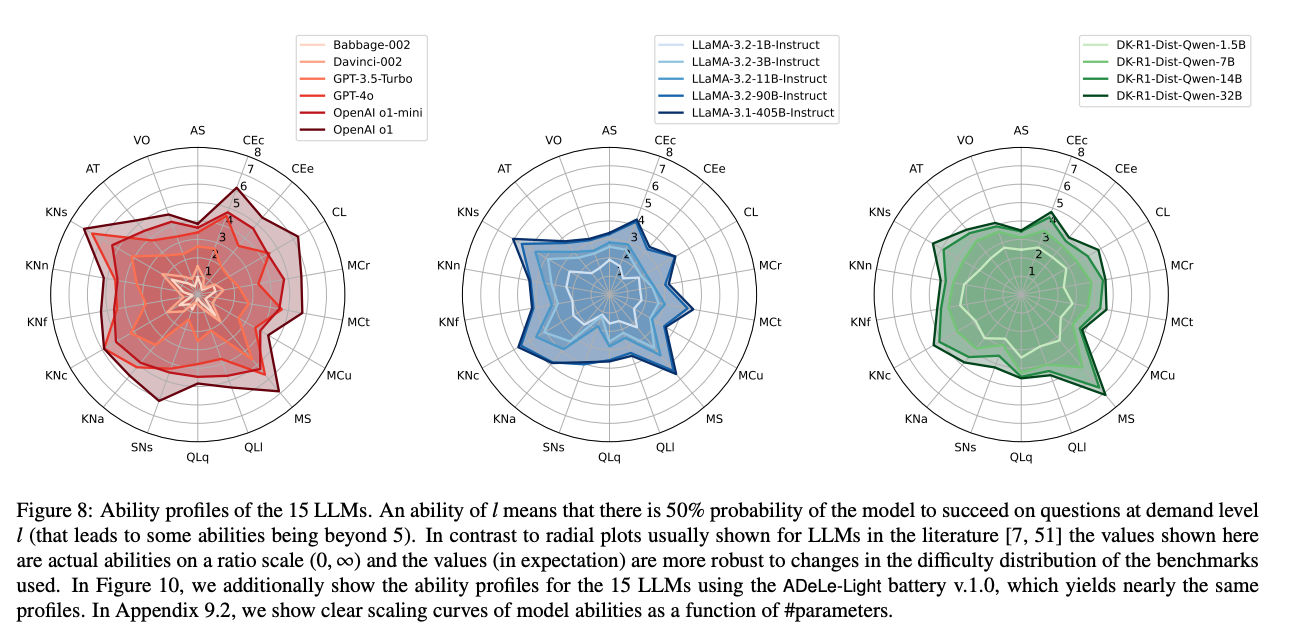
\includegraphics[keepaspectratio]{images/image2.png}}

}

\caption{18-dimensional taxonomy from Lexin Zhou et al. (2025)}

\end{figure}%

\begin{figure}[H]

{\centering \pandocbounded{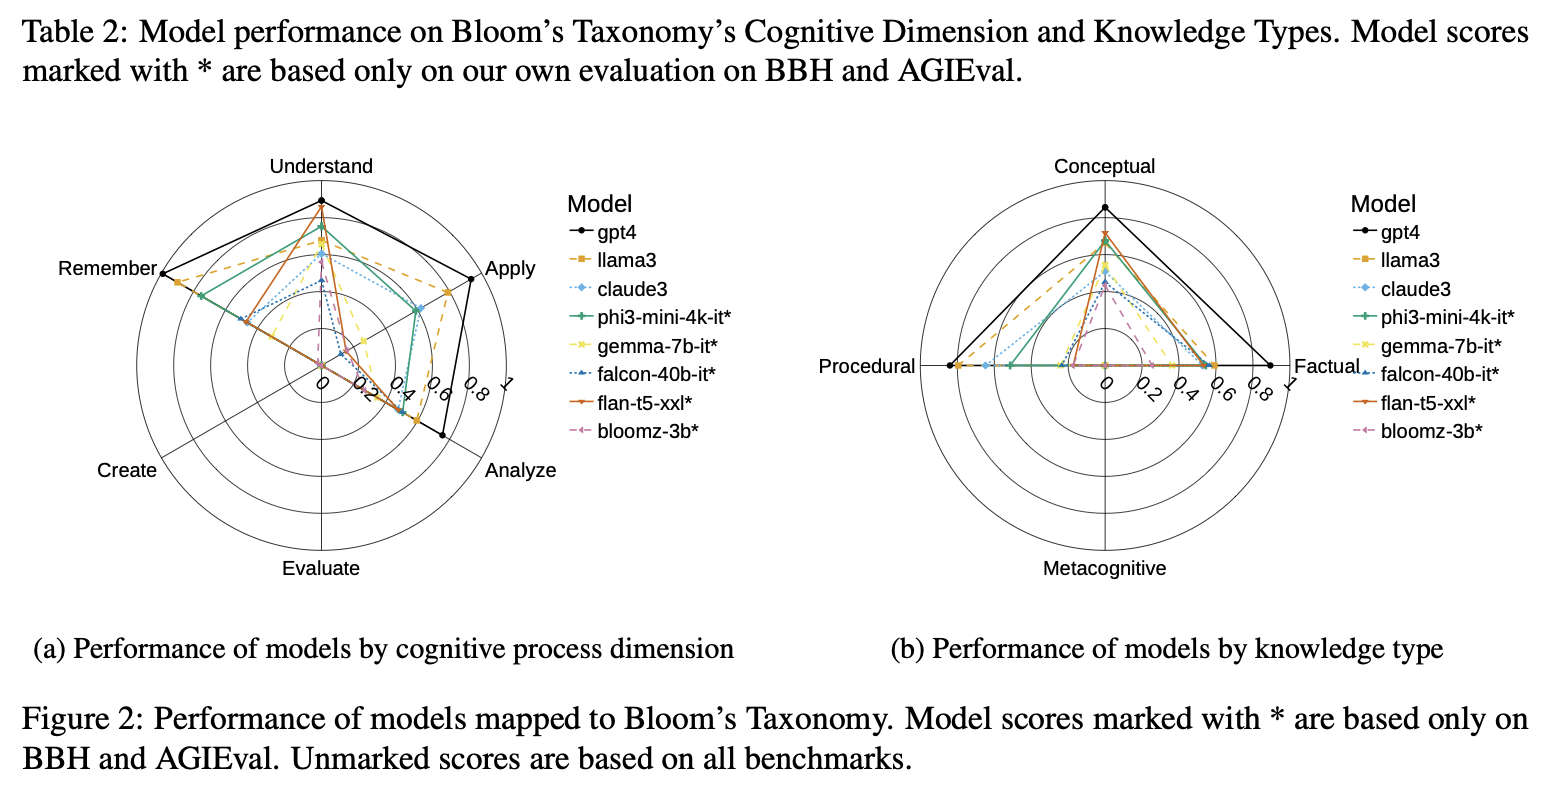
\includegraphics[keepaspectratio]{images/2025-10-19-15-07-10.png}}

}

\caption{10-dimensional taxonomy from Huber and Niklaus (2025)}

\end{figure}%

\begin{figure}[H]

{\centering \pandocbounded{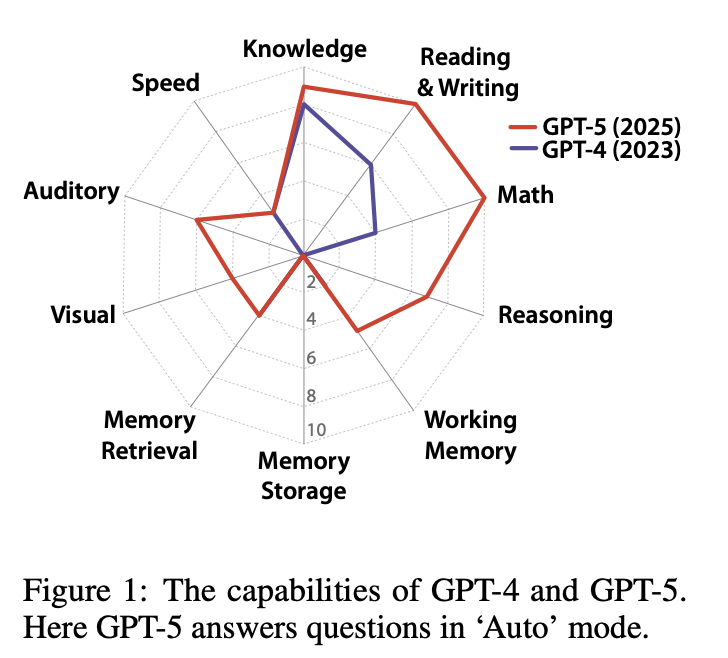
\includegraphics[keepaspectratio]{images/2025-10-19-14-47-17.png}}

}

\caption{10-dimensional taxonomy from Hendrycks et al. (2025)}

\end{figure}%

\begin{figure}[H]

{\centering \pandocbounded{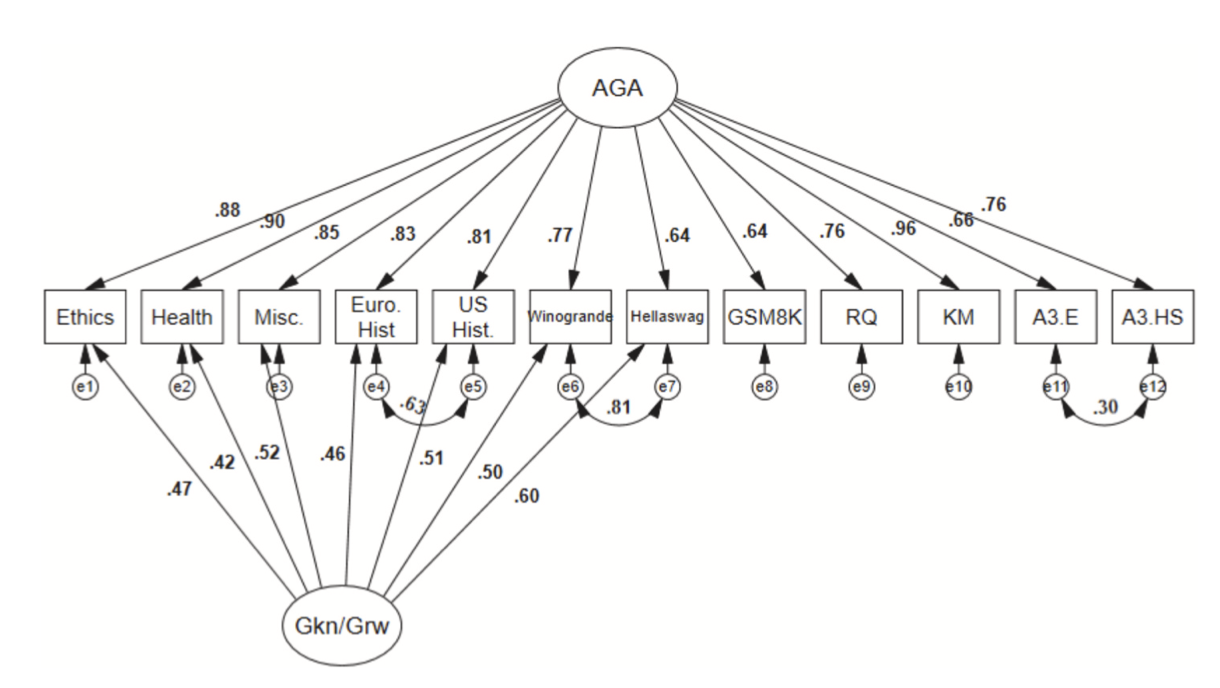
\includegraphics[keepaspectratio]{images/2025-10-21-15-33-31.png}}

}

\caption{From Ilić and Gignac (2024), showing their preferred 2-factor
model}

\end{figure}%

\begin{figure}[H]

{\centering \pandocbounded{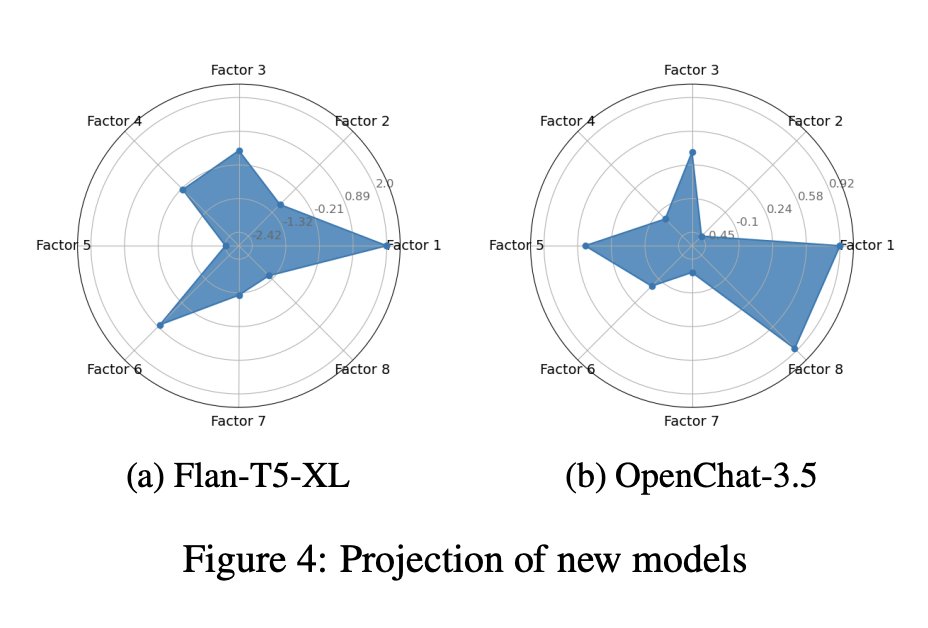
\includegraphics[keepaspectratio]{images/2025-12-05-06-36-08.png}}

}

\caption{From Maimon et al. (2025)}

\end{figure}%

\begin{description}
\item[Some taxonomies of AI capabilities have been proposed but none
have been widely adopted.]
Burnell et al. (2023) look at variation across 29 LLMs and 27 benchmarks
(all prior to GPT-4). The first 3 factors explain 33\%, 31\%, and 17\%
of performance, and they interpret those factors as ``reasoning'',
``comprehension'' and ``core language modeling.'' They say
``capabilities are not monolithic. Instead, they are better explained by
three well-delineated factors that represent reasoning, comprehension
and core language modeling.''

Ilić and Gignac (2024) tested 591 LLMs on 12 different evaluations, as
of March 2024. In their preferred specification the first factor had a
loading of 0.81, implying an R\^{}2 of 0.66. They also found that the
``number of LLM parameters correlated positively with this general
ability.''

Polo et al. (2025) propose a decomposition with three latent factors:
reasoning, knowledge, and instruction-following. However they do not
seem to report overall variance explained by each of the factors.

Maimon et al. (2025) analyze 60 LLMs on 44 tasks, and propose eight
latent factors.

Lexin Zhou et al. (2025) propose an index of 18 different
human-interpretable capabilities (ADeLe). They use an LLM to label
16,000 ``task instances'' from 20 benchmarks, using rubrics to define
each capability. This allows them to predict LLM performance on a task
just based on its content, without any prior LLM successes. The scores
on each dimension are 1-5, they note that they scores approximately
correspond to frequency of achievement among humans, where score \(L\)
will be achieved by \(1/10^{L-1}\) people.\footnote{``an item is at
  level \(l\) if l is the highest number such that, in at least 95\% of
  samples of \(n = 10^l\) individuals, there is at least one correct.''}
response.'')

OECD (2025) organize capabilities across nine dimensions. The criteria
are mostly qualitative, and their scoring is done by a panel of experts
with reference to various benchmark scores. OECD's dimension: Language;
Social interaction; Problem solving; Creativity; Metacognition and
critical thinking; Knowledge, learning and memory; Vision; Manipulation;
Robotic intelligence.

Huber and Niklaus (2025) organize benchmark tasks according to ``Bloom's
Taxonomy'', a heirarchical framework designed to classify educational
learning objectives for humans, with 6 levels: Remember, Understand,
Apply, Analyze, Evaluate, Create. They say there are a lack of
benchmarks to measure the two highest levels (``evaluate'' and
``create'').

Hendrycks et al. (2025) define capabilities along 10 dimensions, based
on the Cattell-Horn-Carroll (CHC) theory of cognitive abilities. They
give testable evals for only some of these capacities.
\item[Many taxonomies are based on components of between-agent
variation.]
Many taxonomies are based on latent factors in variation in performance
in a range of tasks.

Some taxonomies are based on variation among human abilities (e.g.
Hendrycks et al. (2025), Huber and Niklaus (2025)). Some taxonomies are
based on variation across LLM abilities (Burnell et al. (2023), Ilić and
Gignac (2024), Polo et al. (2025), Maimon et al. (2025), Lexin Zhou et
al. (2025)).

A difficulty with both of these approaches is that they are designed to
measure variation \emph{within} one type of agent (LLM or human), not
\emph{between} humans and LLMs. There is reason to expect that there
exist important human-LLM differences that are orthogonal to
within-human or within-LLM variation, e.g.~types of tasks where humans
show little variation, and LLMs show little variation, but there are
large human-LLM differences in ability.\footnote{A similar argument is
  made by Zachary Tidler et
  al.~\href{https://aievaluation.substack.com/p/is-the-definition-of-agi-a-percentage}{here}.}
\end{description}

\subsection{There does appears to be a single latent component of
intelligence across
LLMs}\label{there-does-appears-to-be-a-single-latent-component-of-intelligence-across-llms}

\begin{description}
\item[LLM abilities are highly correlated across models.]
LLM performance is very highly correlated across benchmarks: if model A
beats model B on benchmark X, then it very likely also beats model B on
benchmark Y.

We discuss some literature below which tries to quantify the strength of
this correlation.
\end{description}

\begin{figure}[H]

{\centering \pandocbounded{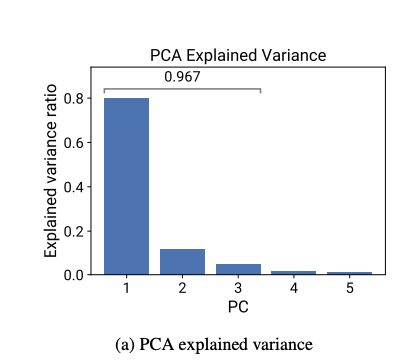
\includegraphics[keepaspectratio]{images/image4.png}}

}

\caption{From Ruan, Maddison, and Hashimoto (2024)}

\end{figure}%

\begin{description}
\item[AI researchers often treat intelligence as a scalar.]
A common sentiment among AI researchers is that it is best to spend time
on making a model generally better, rather than fine-tuning for a
specific case.

This sentiment famously named the ``bitter lesson'' by Sutton (2019):

\begin{quote}
``general methods that leverage computation are ultimately the most
effective, and by a large margin.''
\end{quote}
\item[Much work on ``scaling laws'' treats model intelligence as a
scalar.]
A large part of academic and industry work on AI is spent estimating
``scaling laws'', i.e.~predicting model performance based on various
inputs (e.g.~training compute, training data size, model scale, and
test-time compute). Most work on scaling laws uses a scalar outcome to
represent model intelligence, e.g.~prediction error on a corpus, or
performance on a difficult benchmark. In principle scaling laws could
estimate a \emph{vector} of intelligence outputs however this is
relatively rare, researchers tend to treat a single scalar as a
sufficient proxy for model intelligence.\footnote{polo2025sloth propose
  a decomposition with three latent factors: reasoning, knowledge, and
  instruction-following.}
\item[Some theories of the latent component.]
\hfill
\begin{itemize}
\tightlist
\item
  The Bitter Lesson.

  \hfill
  \begin{itemize}
  \tightlist
  \item
    The ``cognitive core'':
    (\href{https://www.seangoedecke.com/cognitive-core/\#fn-1}{Sean
    Goedeck})
  \item
    The Manifold Hypothesis.
  \item
    The Platonic Representation hypothesis.
  \end{itemize}
\end{itemize}
\end{description}

\hfill\break

\subsection{Latent LLM intelligence appears to be distinct from latent
human
intelligence.}\label{latent-llm-intelligence-appears-to-be-distinct-from-latent-human-intelligence.}

\marginnote{\begin{footnotesize}

\begin{figure}[H]

{\centering \pandocbounded{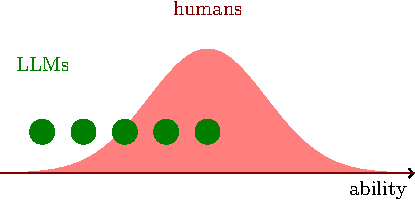
\includegraphics[keepaspectratio]{stylized-facts_files/figure-pdf/unnamed-chunk-2-1.pdf}}

}

\caption{Illustration of LLM vs humans with a single dimension of
ability.}

\end{figure}%

\end{footnotesize}}

\marginnote{\begin{footnotesize}

\begin{figure}[H]

{\centering \pandocbounded{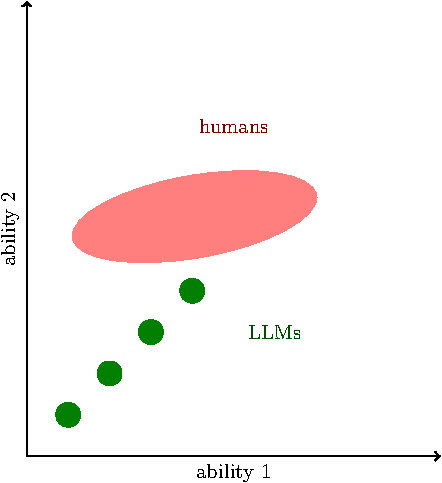
\includegraphics[keepaspectratio]{stylized-facts_files/figure-pdf/unnamed-chunk-3-1.pdf}}

}

\caption{Illustration of LLM vs humans with two dimensions of ability.}

\end{figure}%

\end{footnotesize}}

\begin{description}
\item[Humans have a fairly positive correlation among abilities.]
There is a reasonable correlation among different measures of general
ability (IQ, g-factor).

There is a reasonable correlation between years of education, IQ,
standardized tests score, and wage.
\item[Ideally we would compare human and LLM performance on the same
tasks.]
If we had a full matrix of human and LLM performance we would be able to
compare latent factors of each. Unfortunately there are few datasets
which collect human performance across a range of distinct benchmarks.
\item[We can compare the average human with the average LLM.]
Many benchmarks do report performance for the average or expert human,
so we can make those comparisons. Additionally we can run LLMs on many
human standardized tests and exams.
\item[Latent factors for human and LLM ability appear to be
significantly different.]
Aptitude tests that are predictive for humans are not predictive for
LLMs. GPT-4 was able to get human-level scores at most aptitude tests:
SAT, LSAT, civil service. But GPT-4 did not have the aptitudes passing
such tests implies for humans.

LLMs are able to do tasks no human can: LLMs can translate between pairs
of languages which no human knows (Aymara to Kazakh), can combine
knowledge from two very different domains.
\end{description}

\subsection{\texorpdfstring{There is \emph{some} bottleneck on LLM
abilities, but disagreement about
where}{There is some bottleneck on LLM abilities, but disagreement about where}}\label{there-is-some-bottleneck-on-llm-abilities-but-disagreement-about-where}

\begin{description}
\item[In 2023 many people thought GPT-4 could do a significant fraction
of work:]
\hfill
\begin{itemize}
\item
  Eloundou et al. (2023) estimated that GPT-4 would halve the time
  required to perform a task for between 14\% and 56\% of all tasks in
  the economy.
\item
  Chui et al. (2023) (McKinsey) claimed \emph{``the total percentage of
  hours that could theoretically be automated by integrating
  technologies that exist today \ldots{} {[}is{]} 60--70 percent.''}
\end{itemize}

In retrospect these estimates seem to have been overly optimistic. There
is some missing capability in GPT-4 level ability.
\item[AI researchers are not sure what is the bottleneck.]
\href{https://x.com/karpathy/status/1855659091877937385}{Andrej
Karpathy}, Nov 2024:

\begin{quote}
``Even though by many accounts (evals), LLMs are inching well into top
expert territory (e.g.~in math and coding etc.), you wouldn't hire them
over a person for the most menial jobs. It's an interesting challenge
how we can create evals for all the''easy'' stuff that is secretly hard.
Very long context windows, coherence, autonomy, common sense, multimodal
I/O that works, \ldots{} How do we build good ``menial job'' evals?{}``*
\end{quote}

\href{https://ysymyth.github.io/The-Second-Half/}{Shunyu Yao}, April
2025:

\begin{quote}
``AI has beat world champions at chess and Go, surpassed most humans on
SAT and bar exams, and reached gold medal level on IOI and IMO. But the
world hasn't changed much, at least judged by economics and GDP. I call
this the utility problem, and deem it the most important problem for
AI.''*
\end{quote}
\end{description}

\subsection{There are many candidates for the
bottleneck}\label{there-are-many-candidates-for-the-bottleneck}

Here we list a variety of abilities that LLMs lack, which might explain
the bottleneck to adoption. To make the bottleneck question concrete:
LLMs can pass many tests used to test for human aptitudes (SAT, LSAT,
civil service exams), and many interview questions, yet LLMs clearly
lack the aptitude to perform the associated jobs. Thus there must be
some other missing skill.

\begin{longtable}[]{@{}
  >{\raggedright\arraybackslash}p{(\linewidth - 8\tabcolsep) * \real{0.2892}}
  >{\raggedright\arraybackslash}p{(\linewidth - 8\tabcolsep) * \real{0.3373}}
  >{\centering\arraybackslash}p{(\linewidth - 8\tabcolsep) * \real{0.1928}}
  >{\centering\arraybackslash}p{(\linewidth - 8\tabcolsep) * \real{0.1084}}
  >{\centering\arraybackslash}p{(\linewidth - 8\tabcolsep) * \real{0.0723}}@{}}
\toprule\noalign{}
\begin{minipage}[b]{\linewidth}\raggedright
Capability
\end{minipage} & \begin{minipage}[b]{\linewidth}\raggedright
Benchmark
\end{minipage} & \begin{minipage}[b]{\linewidth}\centering
Apr 2023 (GPT-4)
\end{minipage} & \begin{minipage}[b]{\linewidth}\centering
Dec 2025
\end{minipage} & \begin{minipage}[b]{\linewidth}\centering
Human
\end{minipage} \\
\midrule\noalign{}
\endhead
\bottomrule\noalign{}
\endlastfoot
Deductive reasoning & MATH\footnote{} & 23\% & 98\% & \\
& GPQA\footnote{} & 36\% & 93\% & \\
Information-gathering & GAIA{[}\^{}GAIA{]} & 15\% & 88\% & \\
Accuracy / Hallucination & SimpleQA Verified\footnote{https://arxiv.org/pdf/2509.07968v1
  and https://blog.google/products/gemini/gemini-3/\#gemini-3} &
\textasciitilde30\% & 72\% & \\
Long context & Needle\footnote{https://cloud.google.com/blog/products/ai-machine-learning/the-needle-in-the-haystack-test-and-how-gemini-pro-solves-it}
& 50\% @ 128K & 99.7\% @ 1M & \\
Multimodal inputs & MMMU-Pro \footnote{https://mmmu-benchmark.github.io/\#leaderboard
  and https://blog.google/products/gemini/gemini-3/\#gemini-3} &
\textasciitilde35\% & 81\% & 85\% \\
In-context learning & ARC-AGI\footnote{https://arcprize.org/leaderboard}
& 7\% & 88\% & 77-98\% \\
& ARC-AGI 2\footnote{https://arcprize.org/leaderboard} &
\textasciitilde0\% & 45\% & 98\% \\
\end{longtable}

\begin{longtable}[]{@{}
  >{\raggedright\arraybackslash}p{(\linewidth - 4\tabcolsep) * \real{0.3944}}
  >{\raggedright\arraybackslash}p{(\linewidth - 4\tabcolsep) * \real{0.4507}}
  >{\raggedright\arraybackslash}p{(\linewidth - 4\tabcolsep) * \real{0.1549}}@{}}
\toprule\noalign{}
\begin{minipage}[b]{\linewidth}\raggedright
Bottleneck
\end{minipage} & \begin{minipage}[b]{\linewidth}\raggedright
Benchmarks
\end{minipage} & \begin{minipage}[b]{\linewidth}\raggedright
Benchmarks
\end{minipage} \\
\midrule\noalign{}
\endhead
\bottomrule\noalign{}
\endlastfoot
Continual learning. & Amodei, Karpathy, Hasssabis. & \\
Novel situations & RL generalization, world models. & \\
Interactive decision-making. & & BALROG, 44\% \\
& & \\
\end{longtable}

\begin{description}
\item[Data density.]
Werra (2025) argues that jaggedness is mainly due to availability of
data.
\item[Accuracy.]
LLMs have often made confident false claims (``hallucinations''), and
this has clearly been a barrier to their adoption. This behavior is not
penalized in classic benchmarks which score only right and wrong
answers, and so the LLM has an incentive to guess. Similarly user
pairwise preference does not penalize hallucinations when the user is
not immediately aware of the accuracy of claims.

Benchmarks can test for accuracy in a variety of ways: (1) score based
on confidence; (2) elicit open-ended responses, with a penalty based on
claims that are false or misleading.
\item[Deductive reasoning.]
Many questions involving reasoning are drawn from a fairly stylized
pool, and LLMs historically performed poorly on questions that are
novel, or have misleading associations (``Alice in Wonderland''). Since
the launch of reasoning models in late 2024 LLMs have become far better
at deductive problems.
\item[Novel situations.]
LLMs sometimes fail on problems that are very dissimilar to their
training data (``out of distribution''). Because LLMs are trained on
enormous amounts of data their skills could reflect memorization or
interpolation rather than general intelligence.

Vafa et al. (2024) argue that Transformer-based LLMs can generalize well
along some axes but badly along others. They say ``such incoherence
creates fragility: using a generative model to solve related but subtly
different tasks can lead to failures.'' They propose tests of world
model coherence.
\item[High context.]
Questions on aptitude tests have short prompts, while real-world
problems involve rich context.
\item[Continual learning.]
Typically LLMs have been used in a \emph{stateless} manner, where the
model weights are fixed and only the prompt changes. This means that any
learning about the environment must happen with a separate system, or by
through recursive updates to the prompt. This has been cited by many
people as a critical bottleneck: Karpathy, Hassabis, Altman, Amodei.

\href{https://aipositive.substack.com/p/decoding-deepminds-vision-an-analysis}{Hassabis,
August 2025}

\href{https://www.dwarkesh.com/p/timelines-june-2025}{Dwarkesh Patel,
July 2025}:

\begin{quote}
``the fundamental problem is that LLMs don't get better over time the
way a human would. The lack of continual learning is a huge huge
problem.''
\end{quote}

Dario Amodei, August 2025:

\begin{quote}
``Models learn within the context \ldots{} Maybe we'll train the model
in such a way that it is specialized for learning over the context. You
could, even during the context, update the model's weights \ldots{} So,
there are lots of ideas that are very close to the ideas we have now
that could perhaps do {[}continual learning{]}.''
\end{quote}

\href{https://x.com/polynoamial/status/1994439121243169176}{Noam Brown,
Nov 2025}:

\begin{quote}
``More research breakthroughs are probably needed to achieve AGI/ASI.
(Continual learning and sample efficiency are two examples that
researchers commonly point to.)''
\end{quote}
\end{description}

\href{https://www.youtube.com/watch?v=l3u_FAv33G0&t=3s}{Shane Legg}:

\begin{quote}
``So there are all sorts of things like this {[}continual learning and
visual reasoning{]}, that we currently see. I don't think there are
fundamental blockers on any of these things. \ldots{} So my expectation
is over a number of years these things will all get addressed. But
they're not there yet.''\,''
\end{quote}

\begin{description}
\item[Planning / long-horizon decision-making.]
Dorn et al. (2025) argue that current LLMs are poor at ``sequential
coherence'', they estimate the time-length of ONET tasks as a proxy for
sequential coherence required.
\item[In-context learning.]
Chollet (2019) argues that most benchmarks test for \emph{existing}
skills instead of requiring the agent to learn \emph{new} skills, which
is distinctive for human intelligence. He introduced the Abstraction and
Reasoning Corpus (ARC) task to test for the ability to do skill
acquisition (also sometimes called in-context learning).

LLMs made significant progress on the ARC benchmark, approaching human
levels in 2024. However a new version was introduced (ARC-AGI-2), which
is again relatively straight-forward for a human but difficult for an
LLM.
\item[Multimodal inputs and outputs.]
LLMs primarily operate on text inputs and outputs.
\item[Interactive decision-making.]
Questions on aptitude tests do not require a series of decisions,
navigating an uncertain situation.
\item[Predictability.]
Some people have claimed a bottleneck is the \emph{unpredictability} of
LLM abilities. This can be interpreted in two ways: (1) humans have
systematically biased beliefs about LLM abilities; (2) i.e.~even if LLM
accuracy might be high over a broad class of questions, the accuracy
varies across subclasses. Vafa, Rambachan, and Mullainathan (2024) say
``when the cost of mistakes is high, more capable models can perform
worse on the instances people choose to use them for because they are
not aligned with the human generalization function.''

A related point is that LLMs can be inconsistent, giving qualitatively
different answers to a question when the wording is slightly different.
\item[Cost.]
(\ldots)
\end{description}

I have not added separate category for ``reliability,'' meaning lack of
randomness, because it is relatively to run an LLM in a mostly
deterministic fashion, and so eliminate concerns about randomness.

Other discussions of bottlenecks:

\begin{itemize}
\tightlist
\item
  Toner (2025) discusses reasons for jaggedness: (1) easier vs harder to
  verify tasks; (2) can you put the context in the context window; (3)
  level of adversarialness; (4) cognitive vs physical.
\item
  Heitmann et al. (2025)

  \begin{itemize}
  \tightlist
  \item
    Performance on tasks that are hard to verify
  \item
    Performance on long tasks (that take human workers a long time)
  \item
    Performance in complex environments
  \item
    Sufficiently low error rate
  \item
    Meta-awareness and calibration
  \item
    Adaptability to the deployment environment
  \item
    Continual learning post-deployment
  \item
    Original insights
  \end{itemize}
\end{itemize}

\subsection{There are few forecasts of future
capabilities}\label{there-are-few-forecasts-of-future-capabilities}

\begin{itemize}
\tightlist
\item
  Manifold markets
  https://manifold.markets/SG/eci-2026-epoch-capabilities-index-h
\end{itemize}

\section{LLM Performance on Tasks}\label{llm-performance-on-tasks}

In this section we discuss performance on tasks that have a measurable
output.

\subsection{The time between benchmark introduction and saturation has
been
decreasing}\label{the-time-between-benchmark-introduction-and-saturation-has-been-decreasing}

If we had a cardinal scale of computer intelligence we could talk about
the rate of improvement in a precise way. The best proxy for velocity is
the history of AI benchmarks: new benchmarks are introduced when
computers achieve human-level performance on the old benchmarks
(``saturation'').

{\marginnote{\begin{footnotesize}\pandocbounded{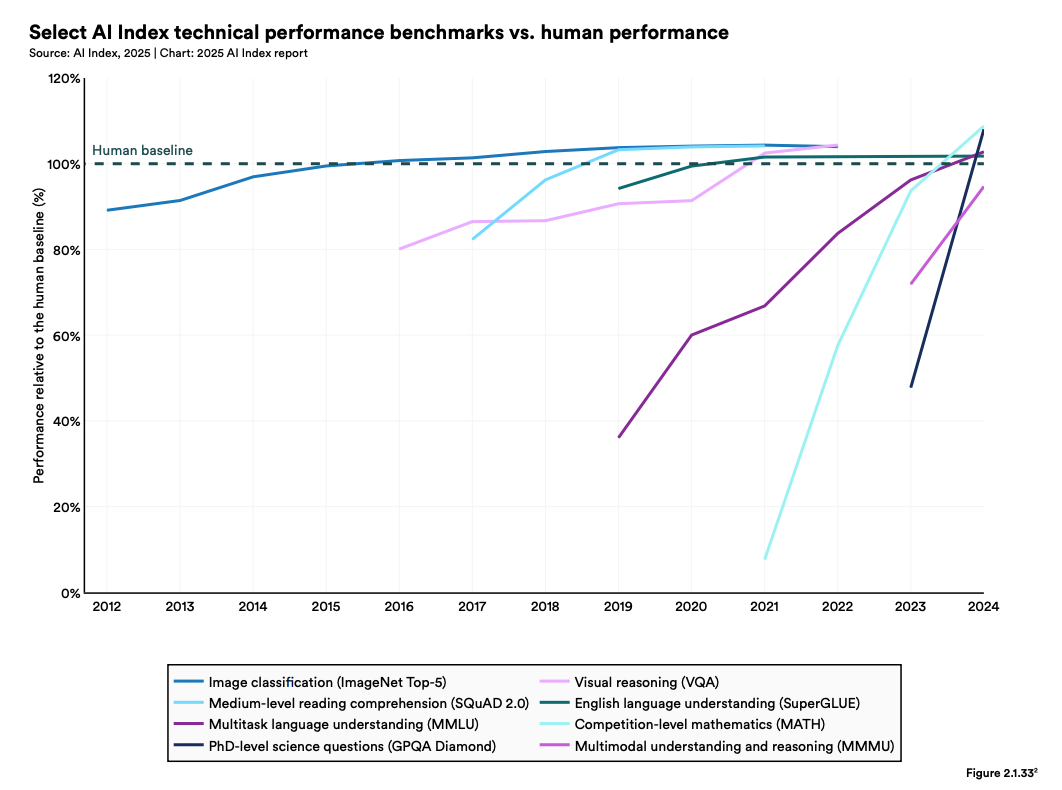
\includegraphics[keepaspectratio]{images/image7.png}}\end{footnotesize}}}
Since 2012 the rate of benchmark saturation seems to be increasing:

\subsection{LLM performance is highly correlated across
benchmarks}\label{llm-performance-is-highly-correlated-across-benchmarks}

\begin{figure}[H]

{\centering \pandocbounded{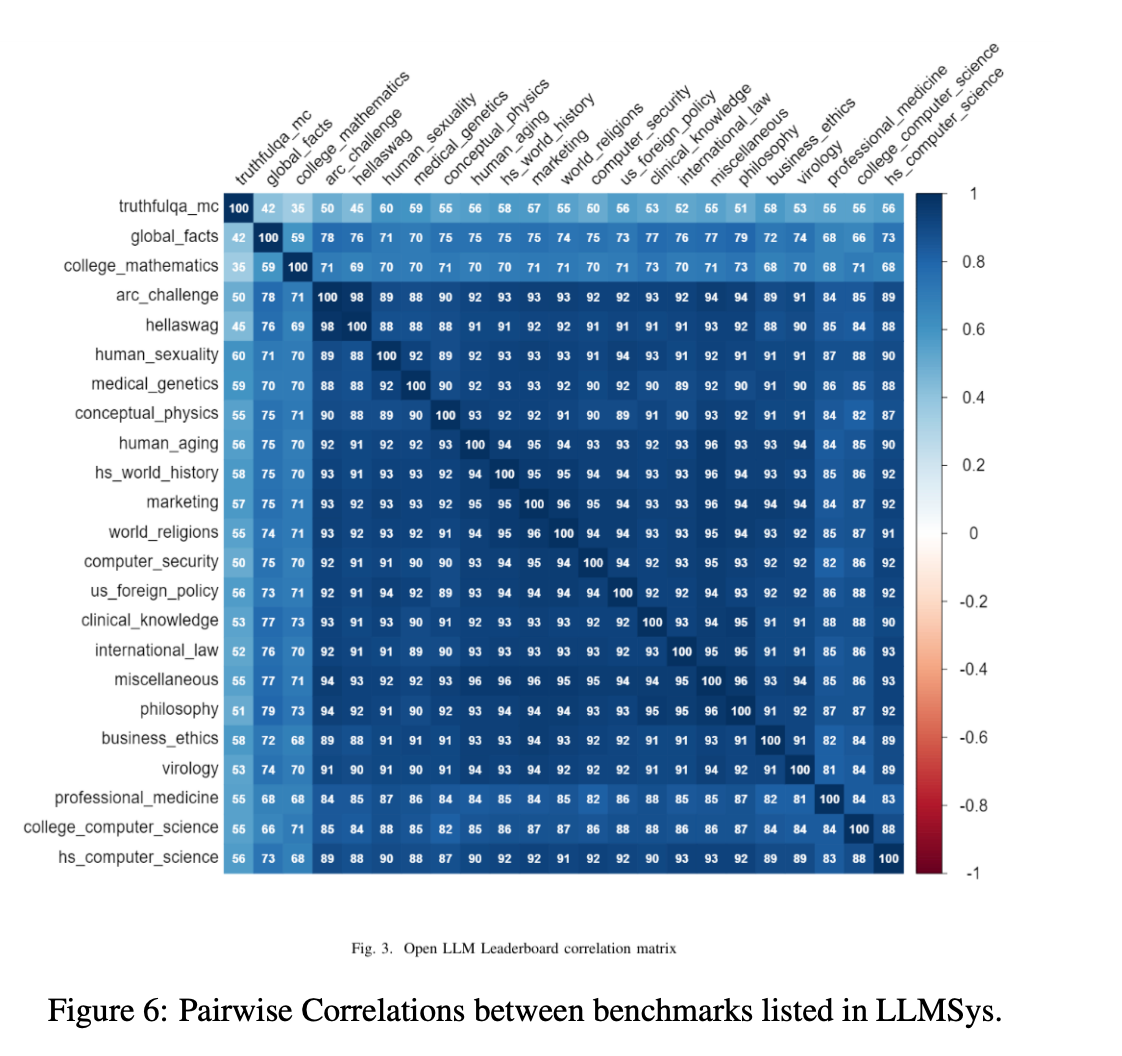
\includegraphics[keepaspectratio]{images/image3.png}}

}

\caption{From Spangher et al. (2024)}

\end{figure}%

\begin{figure}[H]

{\centering \pandocbounded{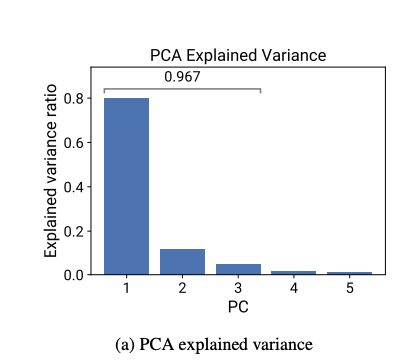
\includegraphics[keepaspectratio]{images/image4.png}}

}

\caption{From Ruan, Maddison, and Hashimoto (2024)}

\end{figure}%

\begin{description}
\item[Frontier models that surpass previous models on one benchmark
usually outperform them on most other benchmarks.]
Spangher et al. (2024) construct an aggregatation across benchmark
scores (MPG = Model Performance and Goodness), which they find is highly
correlated with Elo rating on LMArena. The strongest model in their
dataset is \texttt{o1-preview}.

Ruan, Maddison, and Hashimoto (2024) create ``observational scaling
laws'' from the performance of 77 LLMs (as of May 2024) on 8 benchmarks.
They find the first component explains 80\% of the variation, also that
training compute is highly predictive of this factor (for open models,
which have known scale). They also fit scaling laws for the effect of
inference-time techniques such as Chain-of-Thought and Self-Consistency.

Kipnis et al. (2025) find a small set of questions which are highly
predictive of overall model scores, and that ``a single underlying
common factor whose Spearman correlation with the total score is r=
0.93.''

Zhang, Dominguez-Olmedo, and Hardt (2025) find that differences in model
abilities across benchmarks decline substantially when the models are
given a small fine-tuning on the specific benchmark (train-before-test).

\begin{quote}
``train-before-test reduces the model-score matrix to essentially rank
one, indicating that model potential is dominated by one latent factor,
uncovered by train-before-test.''
\end{quote}

They also find that the latent factor is very highly correlated with
pretraining perplexity.\footnote{Train-before-test also raises rank
  agreement between benchmarks: ``On average, the overall average
  Kendall's τ is 0.52 for direct evaluation and 0.76 for
  train-before-test.''}
\end{description}

\subsection{The best predictor of benchmark performance is training
compute.}\label{the-best-predictor-of-benchmark-performance-is-training-compute.}

There is a well-known literature on ``scaling laws'' finding that
pretraining loss (i.e.~error in predicting the next token) is a
predictable function of the training parameters.

\begin{itemize}
\item
  Kaplan et al. (2020) predict LLM performance in next-token prediction
  error, as a function of model size, dataset size, and training
  compute. They find scaling laws that are reliable across 7 orders of
  magnitude. Their equations implied that model size was the most
  important parameter (not dataset size).\footnote{``Larger models are
    significantly more sample-efficient, such that optimally
    compute-efficient training involves training very large models on a
    relatively modest amount of data and stopping significantly before
    convergence.''}
\item
  J. Hoffmann et al. (2022) revisit scaling laws with more data and a
  different functional form:
  \[\ut{\hat{L}}{loss}(\ut{N}{parameters},\ut{D}{data}) \simeq \utt{E}{irreducible}{loss} + aN^{-.3} + bD^{-.3}\]

  Their fit finds that training data and model size should optimaly
  scale at the same rate. Their model predicted that it would be optimal
  to train a model with much smaller size and larger amount of data,
  compared to existing models. They trained such a model
  (``chinchilla'') and indeed found that it significantly outperformed
  other models with the same compute inputs.
\item
  Choshen, Zhang, and Andreas (2024) surveys scaling-law best-practices
  in 2025, and largely confirms the functional-form and parameters
  proposed in J. Hoffmann et al. (2022).
\end{itemize}

The classical ``scaling laws'' literature predicts the fit on training
loss, meaning next-token prediction error. There is a smaller literature
which predicts performance on task benchmarks (note that these are
usually from a model with post-training):

\begin{figure}[H]

{\centering \pandocbounded{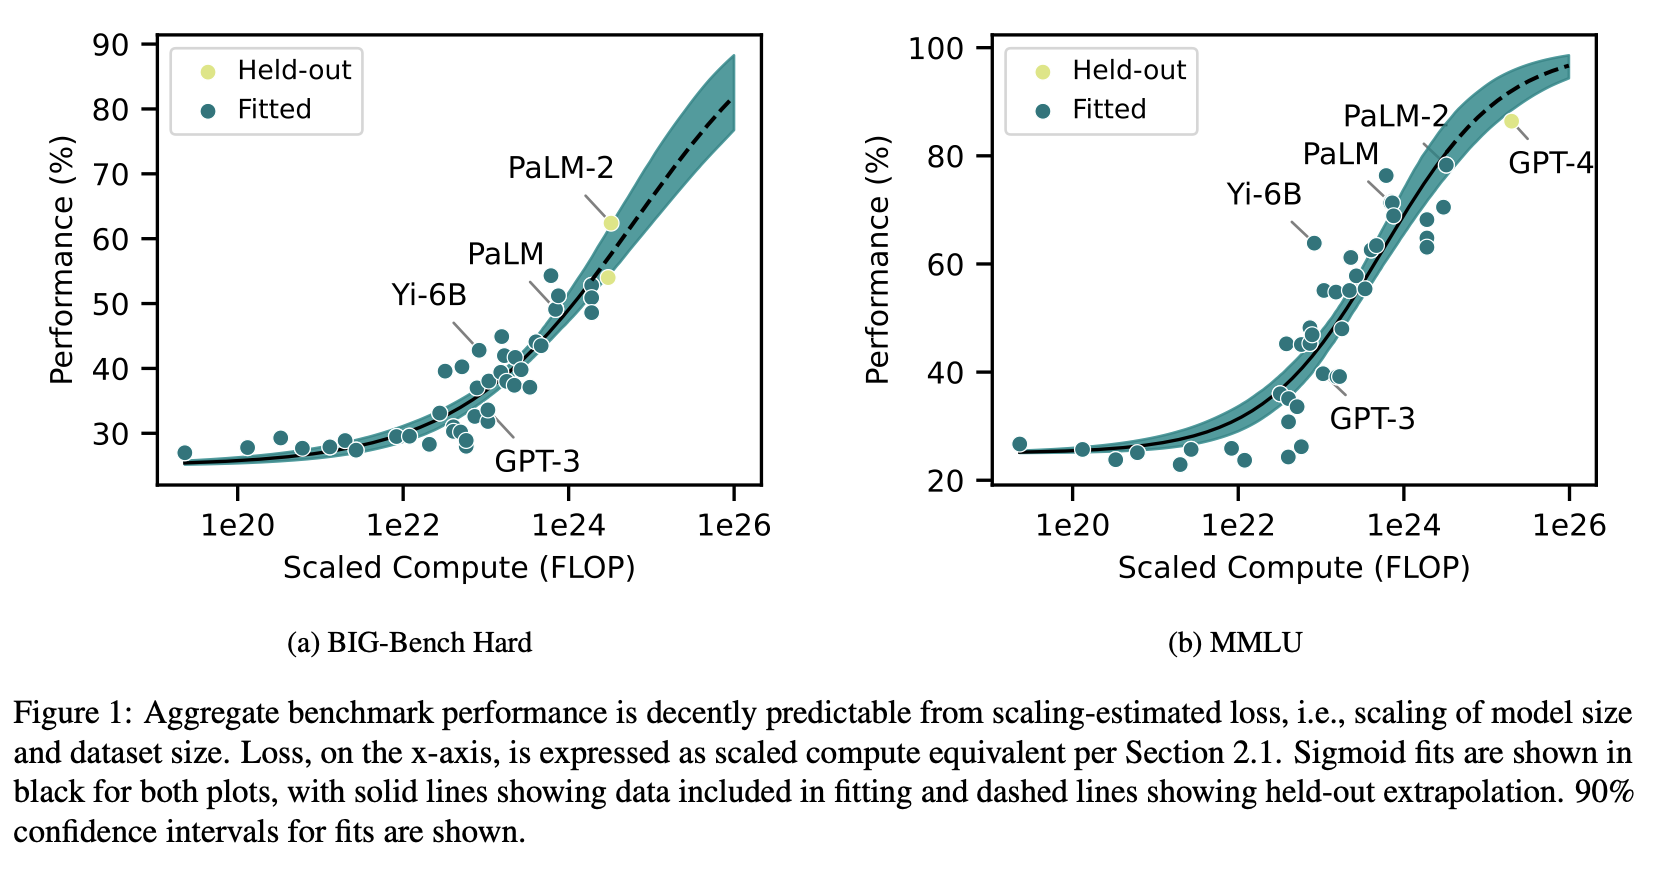
\includegraphics[keepaspectratio]{images/2025-10-21-15-38-28.png}}

}

\caption{From Owen (2024)}

\end{figure}%

\begin{itemize}
\item
  Owen (2024) find that model scale is highly predictive of benchmark
  performance, and the relationship remains relatively stable across
  five orders of magnitude.\footnote{``when extrapolating BIG-Bench Hard
    performance across one order of magnitude in compute, we observe
    average absolute errors of 6 percentage points.''} The strongest
  model in their dataset is GPT-4. This paper also discusses a number of
  previous contributions on benchmark scaling.
\item
  Ruan, Maddison, and Hashimoto (2024) find tight relationships between
  training compute, simple capability measures, and complex downstream
  metrics.
\end{itemize}

\subsection{The effective scale of frontier models has been growing at
around 15X per
year.}\label{the-effective-scale-of-frontier-models-has-been-growing-at-around-15x-per-year.}

The effective scale of frontier models takes into account both the
increase in training compute used as well as the algorthmic efficiency
in utilizing each unit of compute.

\begin{itemize}
\tightlist
\item
  \href{https://epochai.org/trends}{Epoch AI} (Jan 2025) estimate that
  over 2015-2025:

  \begin{enumerate}
  \def\labelenumi{\arabic{enumi}.}
  \tightlist
  \item
    Training compute on frontier LLMs has increased around 5X per year;
  \item
    Algorithmic efficiency increased around 3X per year.
  \end{enumerate}

  \begin{itemize}
  \tightlist
  \item
    Combined, these imply that the ``effective'' compute used on
    frontier models is growing at around 15X per year.
  \end{itemize}
\end{itemize}

\subsection{Benchmark performance significantly improves with test-time
scaling on some
tasks.}\label{benchmark-performance-significantly-improves-with-test-time-scaling-on-some-tasks.}

Test-time scaling (AKA inference-time compute) can be achieved in two
ways:

\begin{enumerate}
\def\labelenumi{\arabic{enumi}.}
\tightlist
\item
  Aggregating multiple models calls (self-consistency AKA majority vote
  Wang et al. (2023), tree-of-thought, etc.)
\item
  Training a model with a variable budget of inference-time tokens
  (``reasoning'' models).
\end{enumerate}

The returns to inference-time compute seem to vary by the nature of the
problem.

Test-time scaling is not a perfect substitute for model scale: Wu et al.
(2025) shows that small models with inference-time compute have
performance that asymptotes below those of large models.

\begin{itemize}
\tightlist
\item
  Beeching, Tunstall, and Rush (2024) find that traditional test-time
  scaling (majority vote, best-of-N, beam search) shows sub-log-linear
  returns on a math problems benchmark.
\item
  You (2025) (Epoch) say that existing evidence from OpenAI and DeepSeek
  shows log-linear relationships between test-time compute and
  performance on benchmarks, and say ``this suggests that performance
  scales with reasoning training in a way similar to pre-training, at
  least for math and coding tasks.''
\item
  Balachandran et al. (2025) compare inference-time compute across a
  variety of tasks and say \emph{``Although inference-time scaling
  improves performance, its effectiveness varies between domains and
  tasks, with diminishing returns as task complexity increases.''}
\end{itemize}

\subsection{Benchmark tasks that are harder for humans are typically
harder for
LLMs.}\label{benchmark-tasks-that-are-harder-for-humans-are-typically-harder-for-llms.}

There is typically a positive correlation betwen the tasks that humans
find more difficult and ones LLMs struggle with the most.

\begin{itemize}
\tightlist
\item
  Lucy Zhou et al. (2024) find a positive correlation between human
  difficulty and AI difficulty.
\item
  Dreyfuss and Raux (2025) find no correlation between human and AI
  success rate across a set of math questions, however note that the
  results are using GPT-3.5.
\end{itemize}

\subsection{LLM performance degrades significantly with context
length.}\label{llm-performance-degrades-significantly-with-context-length.}

As of July 2025, frontier models have an effective context length (where
performance is \textgreater85\% of a short-context task) of around
\textasciitilde16,000 words in the
\href{https://github.com/adobe-research/NoLiMa}{NoLiMa Benchmark}.

\begin{itemize}
\tightlist
\item
  LongBench (Bai et al. (2024)) is a benchmark for long-context
  understanding, found that the best models as of Sep 2024 (o1-preview)
  outperformed human baseliners given 15 minutes by 15\% on short tasks
  (\textless32k context), this dropped to only a 5\% gain for
  long-context tasks (\textgreater128k).
\end{itemize}

\subsection{LLM performance on benchmarks is highly variable within the
same
task.}\label{llm-performance-on-benchmarks-is-highly-variable-within-the-same-task.}

LLMs have stochastic outputs and they often have varying success rates
when the same task is repeated. As a consequence an LLM's average score
on a benchmark can be very different from their best-of-n and worst-of-n
scores (note that if output was deterministic then all three scores
would be identical).

\begin{itemize}
\item
  Renze and Guven (2024) find ``changes in temperature from 0.0 to 1.0
  do not have a statistically significant impact on LLM performance for
  problem-solving tasks''
\item
  Song et al. (2024) say ``we observe that greedy decoding
  {[}temperature=0{]} generally outperforms sampling methods
  {[}temperature\textgreater0{]} for most evaluated tasks.''
\end{itemize}

\subsection{LLM Performance on related sub-tasks is highly
variable.}\label{llm-performance-on-related-sub-tasks-is-highly-variable.}

LLMs generally have much smaller correlations in their ability to
successfully complete similar tasks than humans.

\begin{itemize}
\tightlist
\item
  Dreyfuss and Raux (2025) find that, for a given aggregate SAT score,
  humans have much larger variations across subjects than LLMs.
\end{itemize}

\subsection{LLM performance is sensitive to prompt
wording.}\label{llm-performance-is-sensitive-to-prompt-wording.}

The performance of LLMs on certain benchmarks can vary signficantly
depending on the prompting given to the model.

\begin{itemize}
\item
  Mirzadeh et al. (2024) find that adding irrelevant instructions to a
  prompt significantly lowers performance on grade-school level
  questions. However
  \href{https://andrewmayne.com/2024/10/18/can-you-dramatically-improve-results-on-the-latest-large-language-model-reasoning-benchmark-with-a-simple-prompt/}{Andrew
  Mayne (2024)} shows that this performance penalty disappears when the
  prompt included a warning (``\emph{this might be a trick question
  designed to confuse LLMs with additional information.''}).
\item
  Valmeekam, Stechly, and Kambhampati (2024) finds that translating an
  ordinary problem into an artificial language significantly lowers
  performance on planning problems (e.g.~``mystery blocksworld'' in
  PlanBench). However o1-preview was still able to perform at 50\%.
\item
  Li et al. (2025) find that performance on math problems degrades
  somewhat when reworded. The declines are particularly severe for small
  open-source models.
\end{itemize}

\subsection{Benchmark tasks that take humans longer are typically harder
for
LLMs.}\label{benchmark-tasks-that-take-humans-longer-are-typically-harder-for-llms.}

There is a very strong negative correlation between how long it takes
for a human to complete a task (in logarithmic terms) and the
probability that an LLM will be able to complete it successfully.

\begin{itemize}
\tightlist
\item
  Kwa et al. (2025) find that the longest length of task that a frontier
  LLM has been able to complete with greater than 50\% probability has
  been doubling every seven months over the last six years across a
  range of software engineering, cybersecurity, and general reasoning
  tasks. As of June 2025 it stands at just under two hours. A July 2025
  update from METR shows that the time horizon is similar across other
  benchmarks testing quantitative and analytical skills and whilst there
  are larger differences in other domains (eg. web-browsing tasks) the
  rate of change over time is similar. The relationship between model
  success probability and the length of time it takes a human to
  complete a task is well fit with a logistic curve. The correlation in
  the errors of different models is high (79\% between claude 3.7 and
  o1) even after accounting for task length and average model
  performance suggesting there are features of tasks beyond task length
  with predictive power for model performance.
  {\marginnote{\begin{footnotesize}\pandocbounded{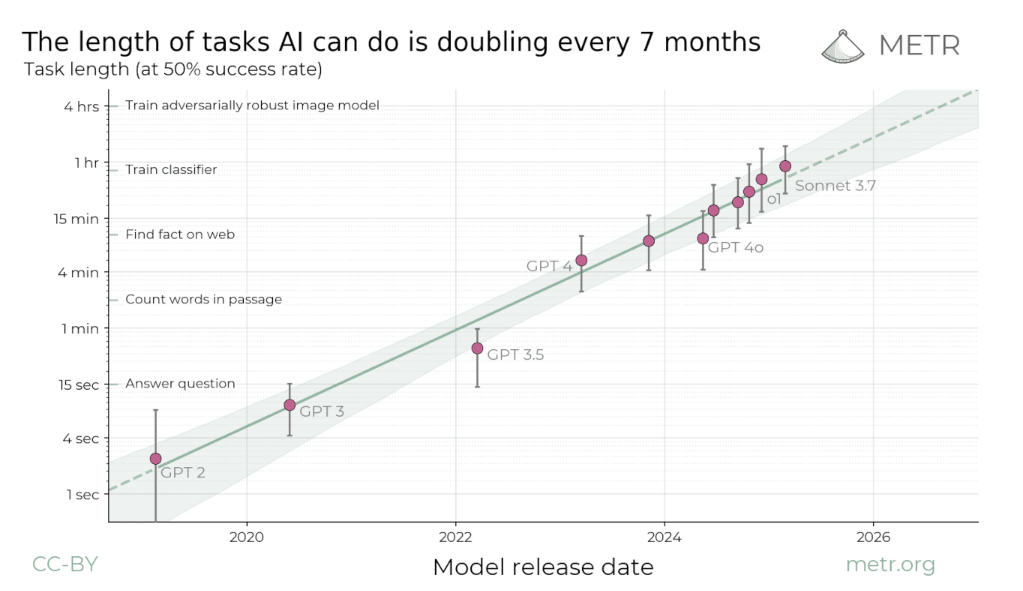
\includegraphics[keepaspectratio]{images/image5.png}}\end{footnotesize}}}
\end{itemize}

{\marginnote{\begin{footnotesize}\pandocbounded{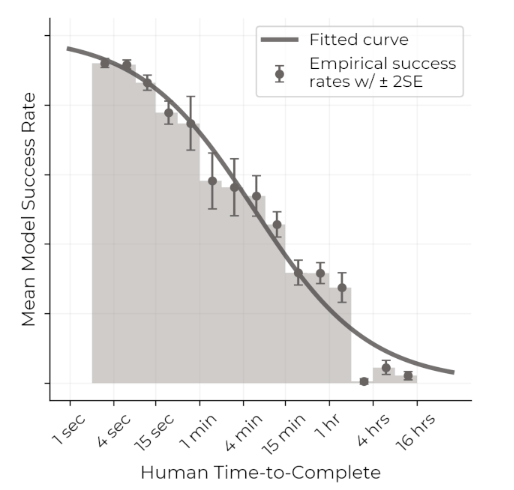
\includegraphics[keepaspectratio]{images/image6.png}}\end{footnotesize}}}

\begin{itemize}
\tightlist
\item
  Ord (2025) argues that LLMs performance degradation over time is
  roughly consistent with a hypothesis that long tasks are random
  combinations of subtasks, each with a constant half-life of success.
\end{itemize}

\subsection{LLMs perform particularly well on math and programming
competition
problems.}\label{llms-perform-particularly-well-on-math-and-programming-competition-problems.}

\begin{itemize}
\tightlist
\item
  Frontier LLMs can outperform the vast majority of competitors in math
  competitions (eg.
  \href{https://www.vals.ai/benchmarks/aime-2025-03-11}{AIME},
  \href{https://arxiv.org/pdf/2103.03874}{MATH}). In a prominent
  programming competition,
  \href{https://arxiv.org/pdf/2501.01257v2}{Codeforces}, o3's
  performance would place it as the 175th ranked competitive programmer
  in the world.
\end{itemize}

\subsection{LLMs show some ability to autonomously complete software
engineering
tasks.}\label{llms-show-some-ability-to-autonomously-complete-software-engineering-tasks.}

\begin{itemize}
\item
  Frontier models can autonomously resolve 75\% of a set of curated
  issues in software systems on github
  (\href{https://openai.com/index/introducing-swe-bench-verified/}{SWE-bench-verified}).
\item
  Frontier models can autonomously produce predictive models on 17\% of
  Kaggle datasets with the same error as a highly skilled data scientist
  (bronze on \href{https://openai.com/index/mle-bench/}{MLE-bench}).
\end{itemize}

\subsection{LLMs are showing ability to improve on algorithmic
tasks.}\label{llms-are-showing-ability-to-improve-on-algorithmic-tasks.}

\begin{itemize}
\tightlist
\item
  Google (2025) reports a 0.7\% saving in Google's worldwide compute
  resources) and aid in the design of new TPU chips.
\end{itemize}

\subsection{LLMs are able to autonomously complete real-world tasks with
significant economic
value.}\label{llms-are-able-to-autonomously-complete-real-world-tasks-with-significant-economic-value.}

Frontier models are able to autonomously complete tasks with high market
value. For instance, an open-source benchmark published by OpenAI finds:

\begin{itemize}
\tightlist
\item
  Miserendino et al. (2025) (SWE-lancer) measures LLM's abilities to
  autonomously complete software engineering and management tasks posted
  on UpWork priced from \$50-\$32,000. As of May 2025, frontier LLMs
  were able to complete 40\% of tasks (i.e.~earn \$400,000 out of \$1M).
\end{itemize}

\subsection{There are few benchmarks in which humans significantly
outperform
computers.}\label{there-are-few-benchmarks-in-which-humans-significantly-outperform-computers.}

It's challenging to find benchmarks in which humans can still outperform
computers. A recent list of
\href{https://docs.google.com/document/d/1cwvepQwLXoZJvgsBpUU5gXmgXml2TOqBRqRV_akfmbA/edit?tab=t.0}{``useful
benchmarks that have human scores beyond AI SOTA''} finds benchmarks
that require UX usage have so far (Nov 2024) resisted saturation.

Even on UX usage benchmarks, the difficulty for LLMs appear to be more
about tooling (which may be more easily rectifiable) than planning
capabilities (the OSWorld paper notes that 75\% of failed attempts are
due to inaccurate mouse clicks rather than planning mistakes).

{\marginnote{\begin{footnotesize}\pandocbounded{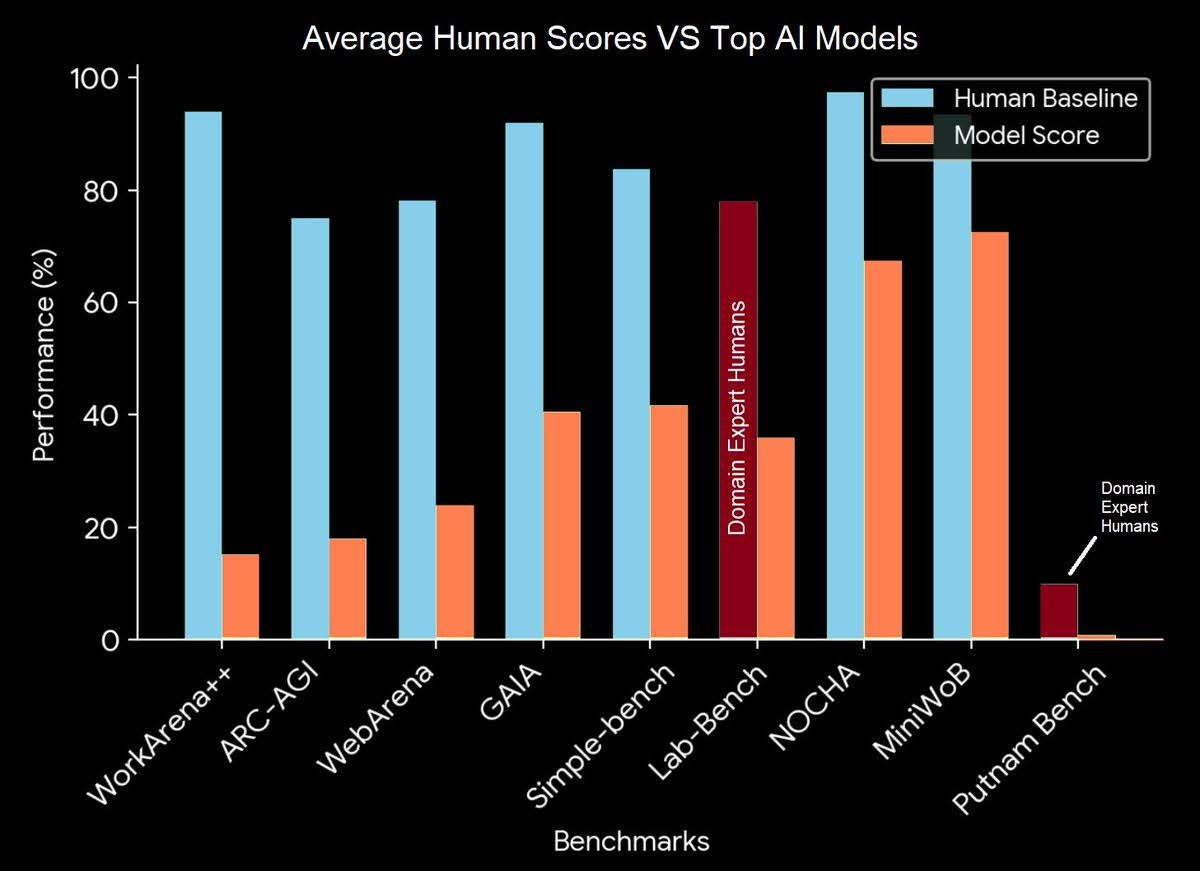
\includegraphics[keepaspectratio]{images/image8.jpg}}\end{footnotesize}}}

\subsection{LLMs show limited ability to perform actions in the real
world.}\label{llms-show-limited-ability-to-perform-actions-in-the-real-world.}

LLMs are able to perform some simple discrete multi-turn tasks in
simulated computer environments but have yet to saturate benchmarks of
simple web-browsing tasks such as
\href{https://hal.cs.princeton.edu/taubench_retail}{Tau-Bench} and
\href{https://arxiv.org/pdf/2404.07972}{OS-world}.

\begin{itemize}
\item
  Anthropic reported on a
  \href{https://www.anthropic.com/research/project-vend-1}{2025 project}
  for Claude to run as a ``shopkeeper'' for a vending machine inside the
  Anthropic offices. They found that the agent hallucinated payment
  accounts, sold items at a loss, and got talked into severe discounts.
\item
  Vending-Bench (Backlund and Petersson (2025)) is a fully simulated
  vending machine setup: frontier agents routinely drive the business to
  bankruptcy within a few in-game weeks, suggesting a lack of long-term
  navigation abilities.
\end{itemize}

\subsection{LLMs show limited ability to play single-player and
multiplayer
games.}\label{llms-show-limited-ability-to-play-single-player-and-multiplayer-games.}

Frontier LLMs struggle playing games that are simple for children to
solve.
{\marginnote{\begin{footnotesize}\pandocbounded{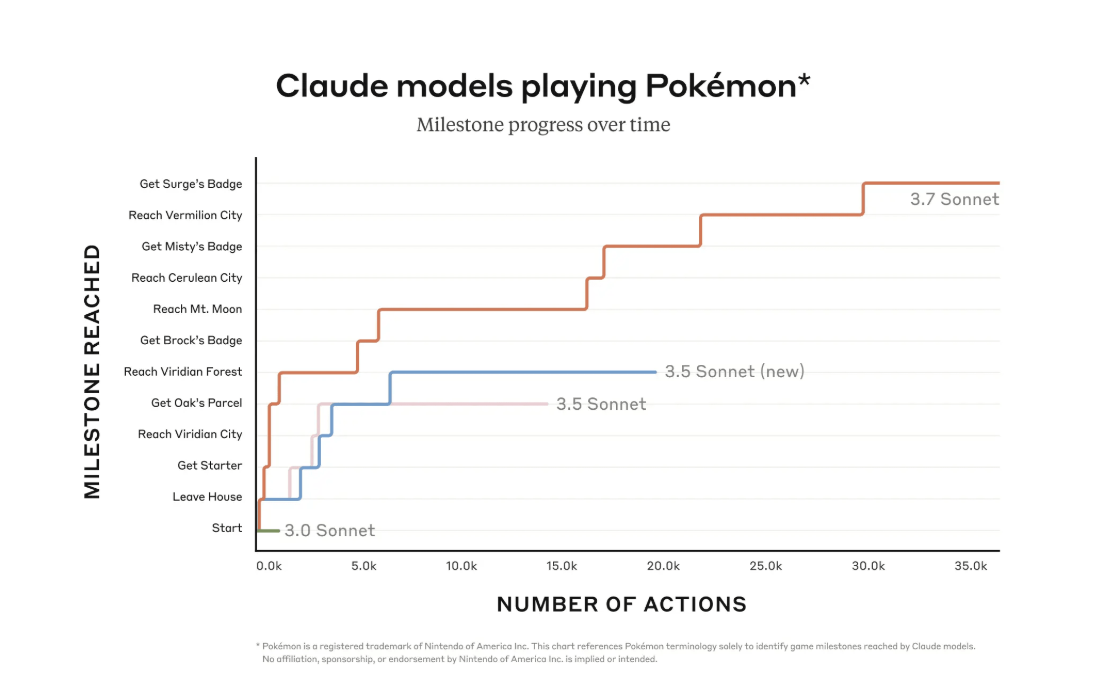
\includegraphics[keepaspectratio]{images/image9.png}}\end{footnotesize}}}

\begin{itemize}
\item
  Paul Calcraft
  \href{https://x.com/paul_cal/status/1890824247792037898}{discusses}
  the state of LLM-gameplaying in early 2025: their performance in
  tic-tac-toe, connect 4, codenames, and chess, is still well below that
  of human experts.
\item
  Payne and Alloui-Cros (2025) find that LLMs are ``highly competitive''
  with the most successful strategies in playing iterated prisoners
  dilemma games.
\item
  LMGame-Bench (Hu et al. (2025)) finds that as of early 2025, LLMs are
  still below human performance across 6 computergames: Sokoban, Super
  Mario Bros, Tetris, 2048, Candy Crush, and Ace Attorney.
\item
  TextQuests (Phan et al. (2025)) find as of August 2025 LLMs are unable
  to solve text-based adventure games that would take human players
  around 30 hours and hundreds of actions to solve without assistance.
  With clues granted recent models are able to make greater progress-
  whilst no model prior to 2025 is able to solve any adventure
  completely, GPT-5 is able to solve 5/25.
\end{itemize}

\subsection{LLMs hallucinate with obscure or long-form
answers.}\label{llms-hallucinate-with-obscure-or-long-form-answers.}

LLMs struggle with reliability and often make up plausible-sounding but
factually incorrect hallucinations.

\begin{itemize}
\tightlist
\item
  GPT-4o and o1-preview hallucinate 30-60 \% of the time when asked
  obscure factual questions, e.g.~``Which Dutch player scored an
  open-play goal in the 2022 Netherlands vs Argentina game in the men's
  FIFA World Cup?'' \footnote{https://assets.ctfassets.net/kftzwdyauwt9/67qJD51Aur3eIc96iOfeOP/71551c3d223cd97e591aa89567306912/o1\_system\_card.pdf}.
\item
  When evaluated on a proprietary benchmark of open-ended questions they
  included incorrect facts in their answers around 80 \% of the time
  \footnote{https://assets.ctfassets.net/kftzwdyauwt9/67qJD51Aur3eIc96iOfeOP/71551c3d223cd97e591aa89567306912/o1\_system\_card.pdf}.
\end{itemize}

However, there has been recent progress made in reducing hallucination
rates. GPT-5, released in August 2025, had six times fewer
hallucinations than o3 as measured by LongFact (2024) and FActScore
(2023).

\subsection{LLMs struggle to give calibrated
answers.}\label{llms-struggle-to-give-calibrated-answers.}

LLMs usually are not aware of what they know or do not know.

\begin{itemize}
\item
  Kadavath et al. (2022) have found that large-parameter models are
  fairly well calibrated in standard benchmarks.
\item
  However a recent OpenAI (2024) study found that models are fairly
  overconfident on tests of obscure facts:\\
  {\marginnote{\begin{footnotesize}\pandocbounded{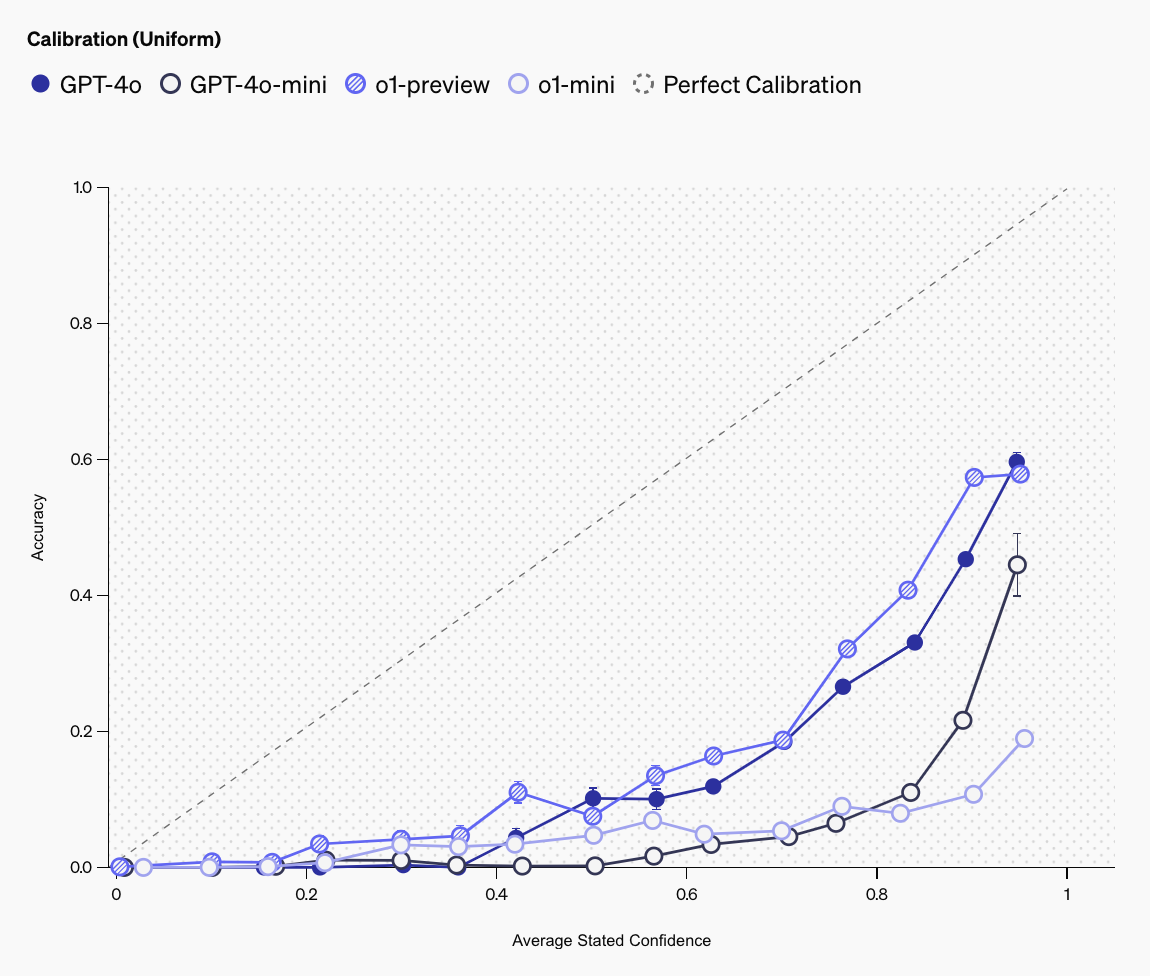
\includegraphics[keepaspectratio]{images/image10.png}}\end{footnotesize}}}
\item
  A Metactulus study in October 2024 found that pro human forecasters
  were ``signficantly better'' than top bots on a set of 113 forecasting
  questions across various domains (eg. politics, economics, the rate of
  technological progress, etc ) and that the bots displayed a positive
  bias (overestimating the likelihood of all events on
  average)\footnote{https://www.metaculus.com/notebooks/28784/aibq3results/}.
\end{itemize}

\section{LLM Augmentation Studies}\label{llm-augmentation-studies}

We define AI ``augmentation'' as the effect of combined AI and human
ability, compared to human-alone ability. These are sometimes also
called ``uplift'' or ``centaur'' studies.

\subsection{The productivity effects of LLM augmentation varies
widely}\label{the-productivity-effects-of-llm-augmentation-varies-widely}

These RCTs compare behavior of workers with and without access to an AI
system:

\begin{figure*}

\begin{longtable}[]{@{}
  >{\raggedright\arraybackslash}p{(\linewidth - 6\tabcolsep) * \real{0.0664}}
  >{\raggedright\arraybackslash}p{(\linewidth - 6\tabcolsep) * \real{0.1063}}
  >{\raggedright\arraybackslash}p{(\linewidth - 6\tabcolsep) * \real{0.1163}}
  >{\raggedright\arraybackslash}p{(\linewidth - 6\tabcolsep) * \real{0.7110}}@{}}
\toprule\noalign{}
\begin{minipage}[b]{\linewidth}\raggedright
Domain
\end{minipage} & \begin{minipage}[b]{\linewidth}\raggedright
Reference(s)
\end{minipage} & \begin{minipage}[b]{\linewidth}\raggedright
Productivity
\end{minipage} & \begin{minipage}[b]{\linewidth}\raggedright
Quote
\end{minipage} \\
\midrule\noalign{}
\endhead
\bottomrule\noalign{}
\endlastfoot
Software engineering & Cui et al. (2024) & & \\
& M. Hoffmann et al. (2025) & & \\
& Gao (2024) & +9\% pull requests/day & ``Accenture developers saw an
8.69\% increase in pull requests \ldots{} a 15\% increase to the pull
request merge rate \ldots{} an 84\% increase in successful builds
\ldots{} developers accepted around 30\% of GitHub Copilot's
suggestions.'' \\
& Peng et al. (2023) & +126\% tasks/minute & ``The treatment group, with
access to the AI pair programmer, completed the task 55.8\% faster than
the control group.'' (implies +126\% tasks/minute) \\
& Becker et al. (2025) & -16\% tasks/minute & ``Allowing AI actually
increases completion time by 19\%---AI tooling slowed developers down.''
(implies -16\% tasks/minute) \\
Consultants & Dell'Acqua et al. (2023) & & \\
Writing tasks & Noy and Zhang (2023) & & \\
Call centre workers & Brynjolfsson, Li, and Raymond (2023) & +15\%
issues/hour & ``Access to AI assistance increases worker productivity,
as measured by issues resolved per hour, by 15\% on average, with
substantial heterogeneity across workers.'' \\
Translators & Merali (2024) & +24\% translations/minute & ``With access
to any AI model {[}time taken{]} was reduced \ldots{} {[}by{]} 31.1\%.''
(=+24\% translations/minute) \\
Entrepreneurs & Otis et al. (2024) & no statistically significant effect
& \\
Legal tasks & Choi, Monahan, and Schwarcz (2023) & +12\%--+32\%
tasks/minute & \\
Radiology & Agarwal et al. (2024) & +0.2\% & \\
& & & \\
\end{longtable}

\end{figure*}%

\begin{figure}[H]

{\centering \pandocbounded{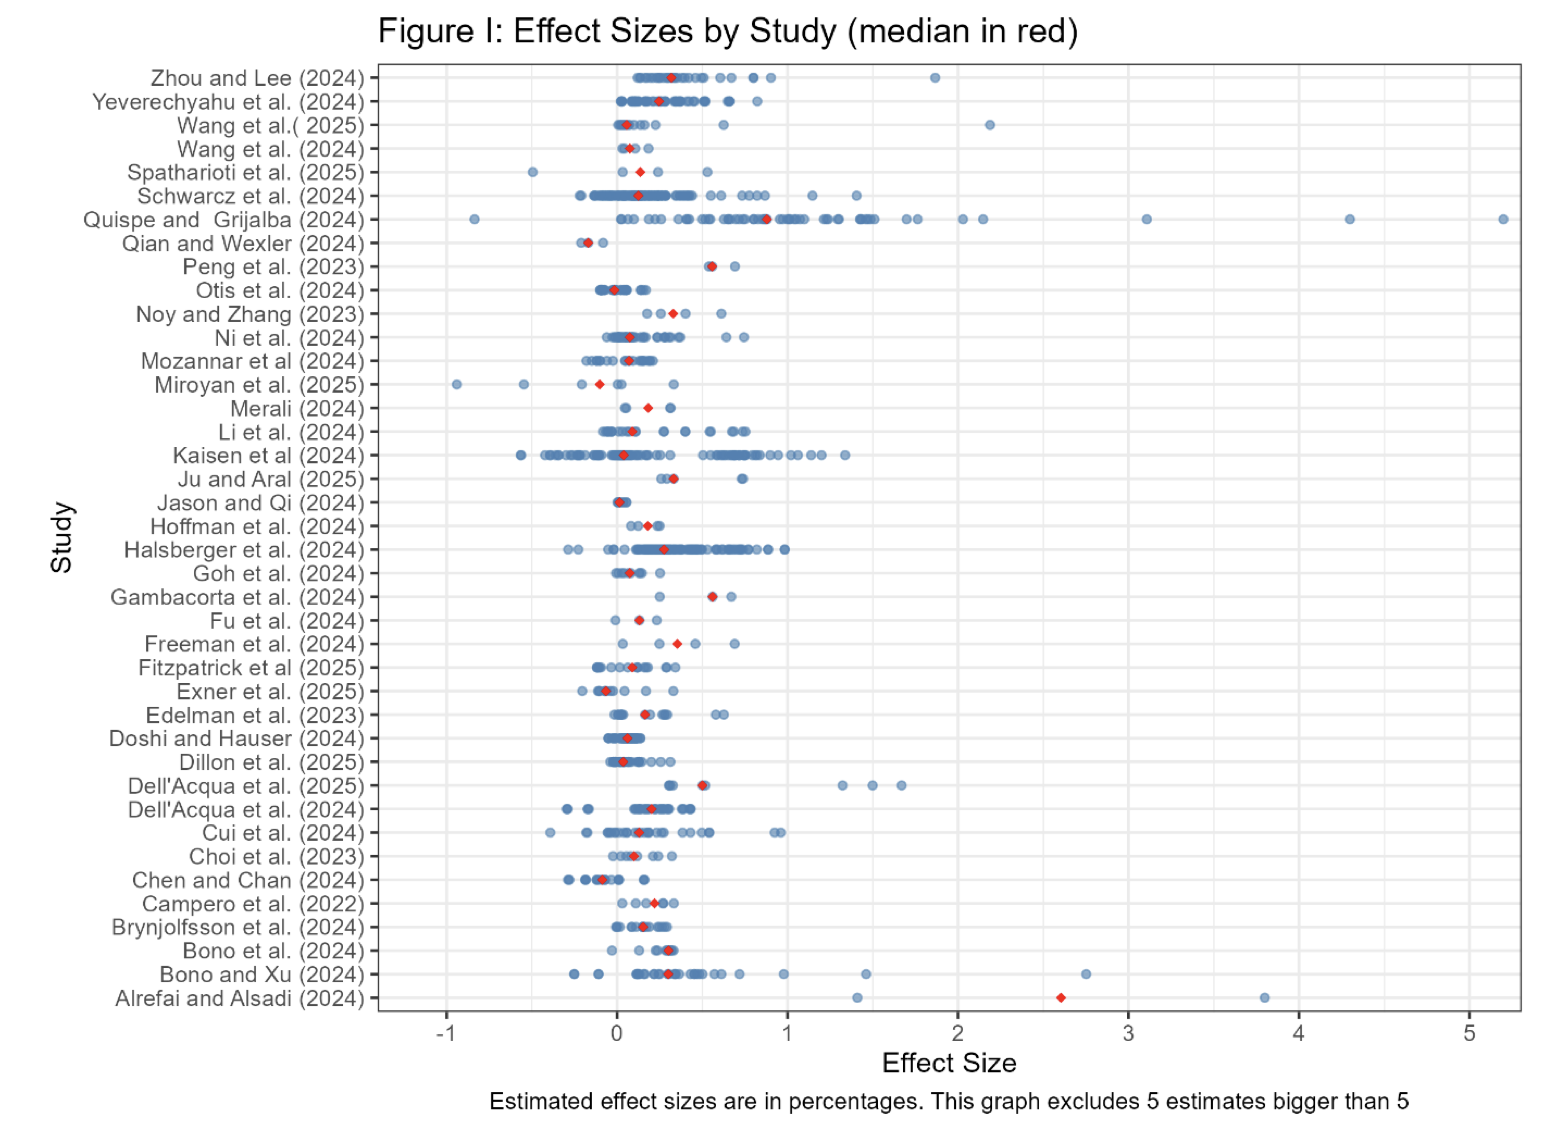
\includegraphics[keepaspectratio]{images/2025-10-20-09-27-43.png}}

}

\caption{Distribution of effect sizes, from Coupé and Wu (2025)}

\end{figure}%

Coupé and Wu (2025) survey 45 studies of the impact of genAI tools on
productivity, with an average productivity effect of +17\%, however with
much variation. They also find strong signs of selection in estimates,
suggesting the true effects are likely smaller.

Vaccaro, Almaatouq, and Malone (2024) survey 106 studies published
between 2020 and 2023. They found:

\begin{quote}
on average, human--AI combinations performed significantly worse than
the best of humans or AI alone (Hedges' g = −0.23; 95\% confidence
interval, −0.39 to −0.07). Second, we found performance losses in tasks
that involved making decisions and significantly greater gains in tasks
that involved creating content. Finally, when humans outperformed AI
alone, we found performance gains in the combination, but when AI
outperformed humans alone, we found losses.
\end{quote}

\subsection{There is some evidence of larger effects on
lower-productivity
workers}\label{there-is-some-evidence-of-larger-effects-on-lower-productivity-workers}

The following RCTs find that augmentation has a larger relative effect
on workers with lower pre-experimental productivity levels:

\begin{itemize}
\tightlist
\item
  Brynjolfsson, Li, and Raymond (2023): ``Less experienced and
  lower-skilled workers improve both the speed and quality of their
  output while the most experienced and highest-skilled workers see
  small gains in speed and small declines in quality.''
\item
  Noy and Zhang (2023): ``there is a correlation of 0.49 between a
  control participant's average grade on the first task and their
  average grade on the second task. In the treatment group, initial
  inequalities are half-erased by the treatment: the correlation between
  first-task and second-task grades is only 0.25''
\item
  Choi, Monahan, and Schwarcz (2023)
\item
  Peng et al. (2023)

  \begin{itemize}
  \tightlist
  \item
    Magnitude: ``The treatment group, with access to the AI pair
    programmer, completed the task 55.8\% faster than the control
    group.''
  \end{itemize}
\end{itemize}

\subsection{There are few benchmarks of
augmentation}\label{there-are-few-benchmarks-of-augmentation}

\begin{itemize}
\tightlist
\item
  Haupt and Brynjolfsson (2025) argues for creating standardized
  benchmarks of augmentation/uplift they refer to as ``centaur''
  evaluations.
\end{itemize}

\subsection{Human + AI teams do not reliably outperform the better of
human or AI performance
individually}\label{human-ai-teams-do-not-reliably-outperform-the-better-of-human-or-ai-performance-individually}

\begin{itemize}
\item
  Vaccaro, Almaatouq, and Malone (2024) across 16 decision-making tasks
  hybrid pairs under-performed the top human-or-AI agent in 70 \% of
  cases, though they sometimes added creative diversity.
\item
  Agarwal et al. (2024) in a radiology-diagnosis experiment, human--AI
  collaboration improved accuracy by only 0.2 pp over AI-only and did
  \textbf{not} outperform selective automation.
\end{itemize}

\subsection{Humans often misperceive the abilities of
LLMs.}\label{humans-often-misperceive-the-abilities-of-llms.}

\begin{itemize}
\item
  Dreyfuss and Raux (2025) find ``projection of human difficulty onto AI
  predictably distorts subjects' beliefs''.
\item
  Vafa, Rambachan, and Mullainathan (2024) say ``We collect a dataset of
  19K examples of how humans make generalizations across 79 tasks from
  the MMLU and BIG-Bench benchmarks \ldots{} based on short
  interactions, humans reach overconfident conclusions about the
  capabilities of the largest models.''
\item
  Agarwal et al. (2024) find that radiologists do not use AI data
  efficiently.
\item
  Becker et al. (2025) find that experienced software engineers
  inaccurately believe that they have experienced productivity speedups
  when using AI tools.
\end{itemize}

However there are limits on what these studies can tell us.

They measure short-run outcomes, but in most jobs the performance cannot
be easily measured with short-run outcomes. E.g. it is challenging to
interpret experiments which measure the effect of LLMs on office
workers' measurable activities (emails, pull requests).

The effects of AI are highly heterogenous across tasks and occupations.

It is difficult to extrapolate the results into the future given the
advance in model capabilities (Merali (2024) attempts to fit model scale
to productivity.)

These experiments often do not measure the ability of models to perform
tasks autonomously.

These experiments do not incorporate general equilibrium effects.

A similar discussion of the limitations of augmentation experiments is
made in a recent
\href{https://empiricrafting.substack.com/p/sci-fi-economics?r=365z3v&utm_campaign=post&utm_medium=web&triedRedirect=true}{Andrey
Fradkin blog post}.

\section{Implications for LLM Economic
Impact}\label{implications-for-llm-economic-impact}

\subsection{The price of inference for a fixed level of capability has
been falling at 10X/year or
faster.}\label{the-price-of-inference-for-a-fixed-level-of-capability-has-been-falling-at-10xyear-or-faster.}

\begin{figure}[H]

{\centering \pandocbounded{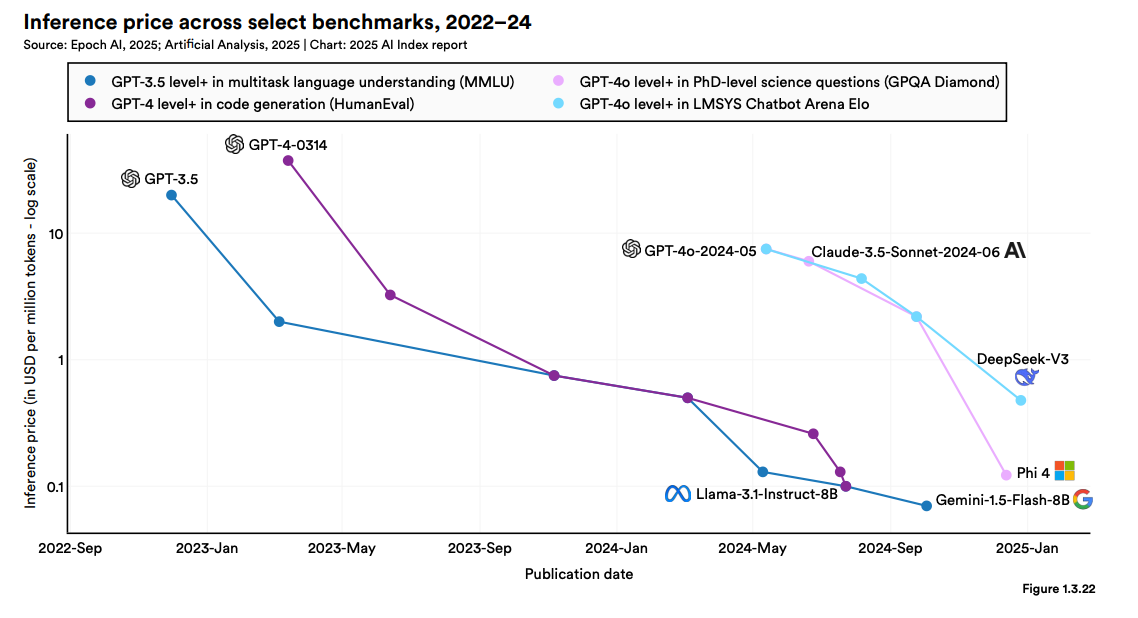
\includegraphics[keepaspectratio]{images/image15.png}}

}

\caption{From Maslej et al. (2025)}

\end{figure}%

\begin{itemize}
\tightlist
\item
  Maslej et al. (2025) estimate that inference costs, for a given level
  of intelligence, fell over 2022-2024 at annual rates exceeding
  10X/year.
\end{itemize}

{\marginnote{\begin{footnotesize}\pandocbounded{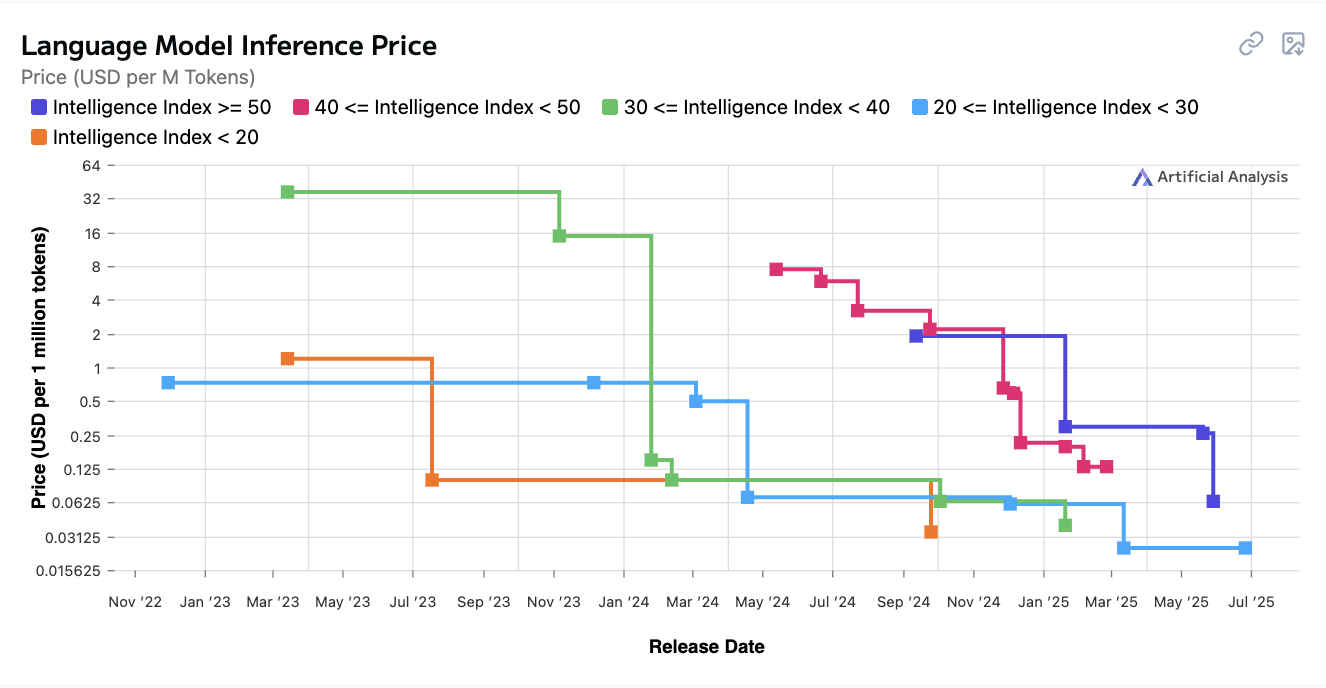
\includegraphics[keepaspectratio]{images/2025-07-16-22-25-34.png}}\end{footnotesize}}}

\begin{itemize}
\tightlist
\item
  \href{https://artificialanalysis.ai/trends}{Artificial Analysis} track
  per-token price trends since 2022: within each tier of model
  intelligence, the price typically halves every few months.
\end{itemize}

\begin{figure}[H]

{\centering \pandocbounded{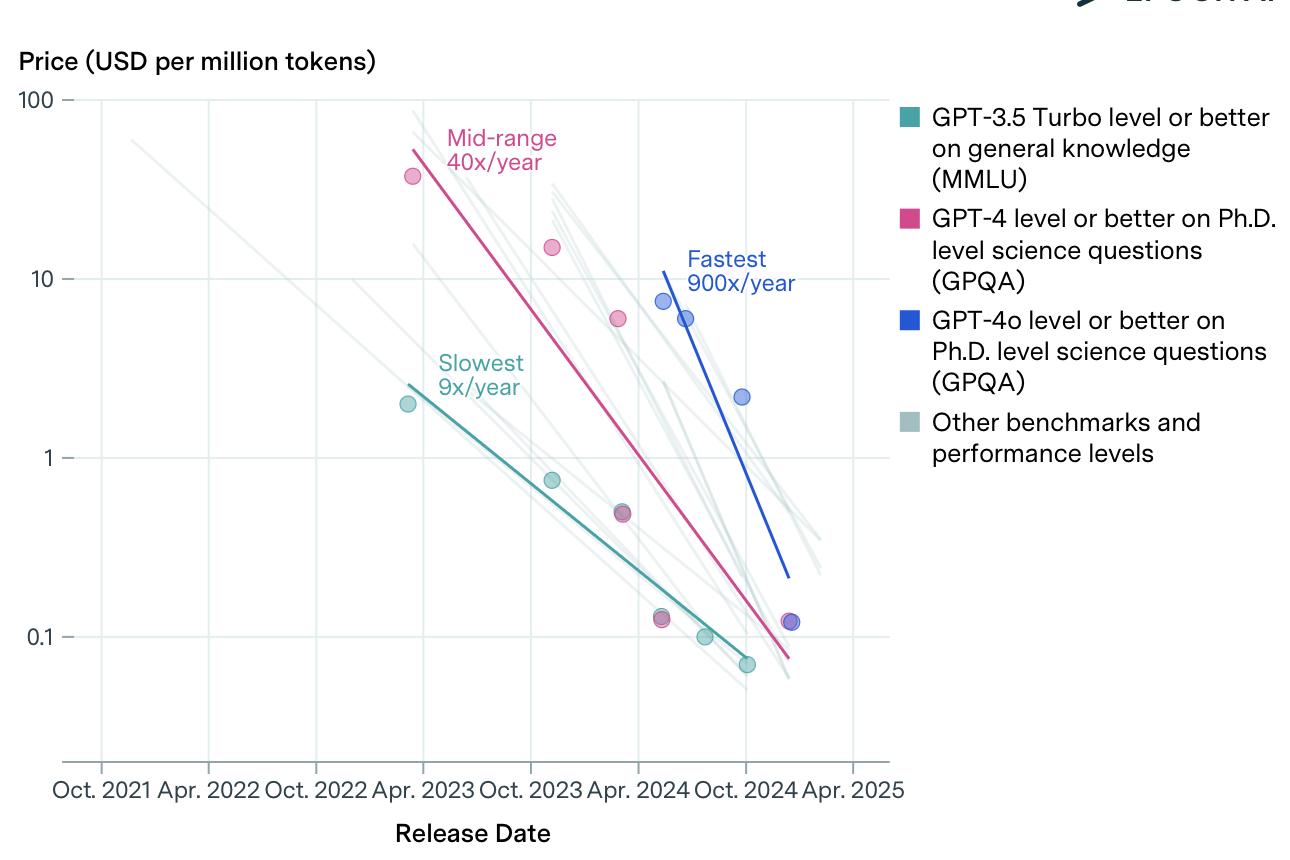
\includegraphics[keepaspectratio]{images/2025-10-20-12-31-11.png}}

}

\caption{From Cottier et al. (2025)}

\end{figure}%

\begin{itemize}
\tightlist
\item
  Cottier et al. (2025) find price declines over 2023-2025 from between
  9X/year (for gpt-3.5 ability on MMLU), up to 900X/year (for gpt-4o
  ability on GPQA).
\end{itemize}

\subsection{The cost of inference for frontier capabilities has remained
roughly
stable.}\label{the-cost-of-inference-for-frontier-capabilities-has-remained-roughly-stable.}

The retail price of intelligence is determined by the compute
requirement, the cost of compute, and the markup. Also note that the
per-token price can be very different from the per-request price for
reasoning models.

\begin{itemize}
\item
  \href{https://artificialanalysis.ai/trends}{Artificial Analysis} show
  that the per-token price of frontier intelligence over time shows no
  clear trend (the chart above). Note that this chart does not include
  the current highest-tier models, as of July 16 Grok4 has a price of
  \$6/M tokens.
\item
  The price of compute has been relatively stable over 2023-2025, with
  A100 priced at around \$2/hour (see Lambda Cloud pricing Lambda Labs
  (2025)).
\end{itemize}

\subsection{Inference costs of serving a model are now roughly
proportional to the initial training
costs.}\label{inference-costs-of-serving-a-model-are-now-roughly-proportional-to-the-initial-training-costs.}

There is a tradeoff between training cost and inference cost through
model size. Larger models will have higher inference costs.

\begin{itemize}
\tightlist
\item
  Erdil (2024) concludes AI labs should spend ``comparable resources in
  training and running inference''.
\end{itemize}

\subsection{LLMs are almost always cheaper than
humans}\label{llms-are-almost-always-cheaper-than-humans}

METR (2024) compare the cost of humans and LLMs to do a variety of
tasks, they say ``when agents \emph{can} do a task, they can often do so
at a fraction of the cost of humans.''

\begin{figure}[H]

{\centering \pandocbounded{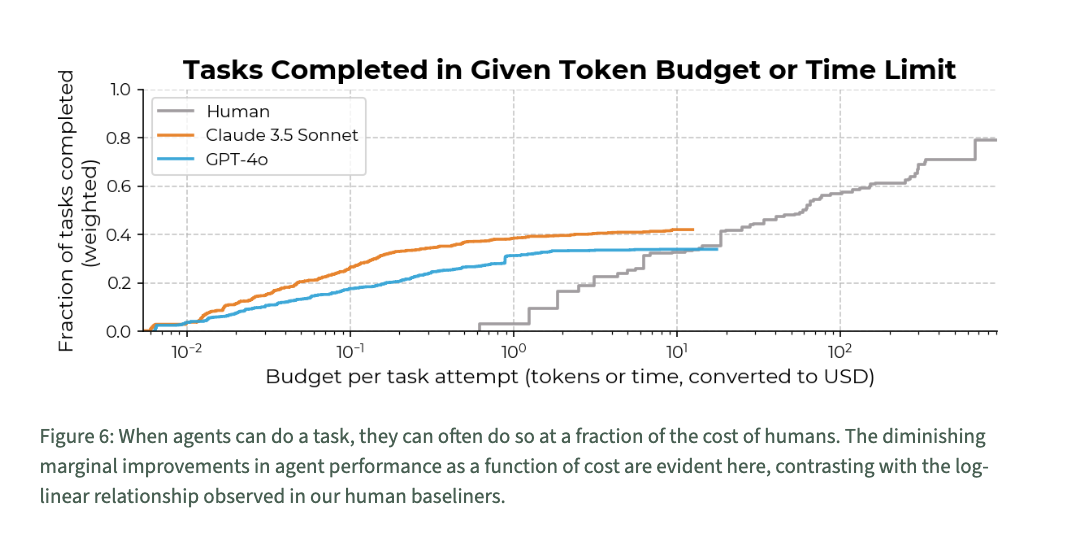
\includegraphics[keepaspectratio]{images/image16.png}}

}

\caption{From METR (2024)}

\end{figure}%

Similarly METR (2025) finds:

\begin{figure}[H]

{\centering \pandocbounded{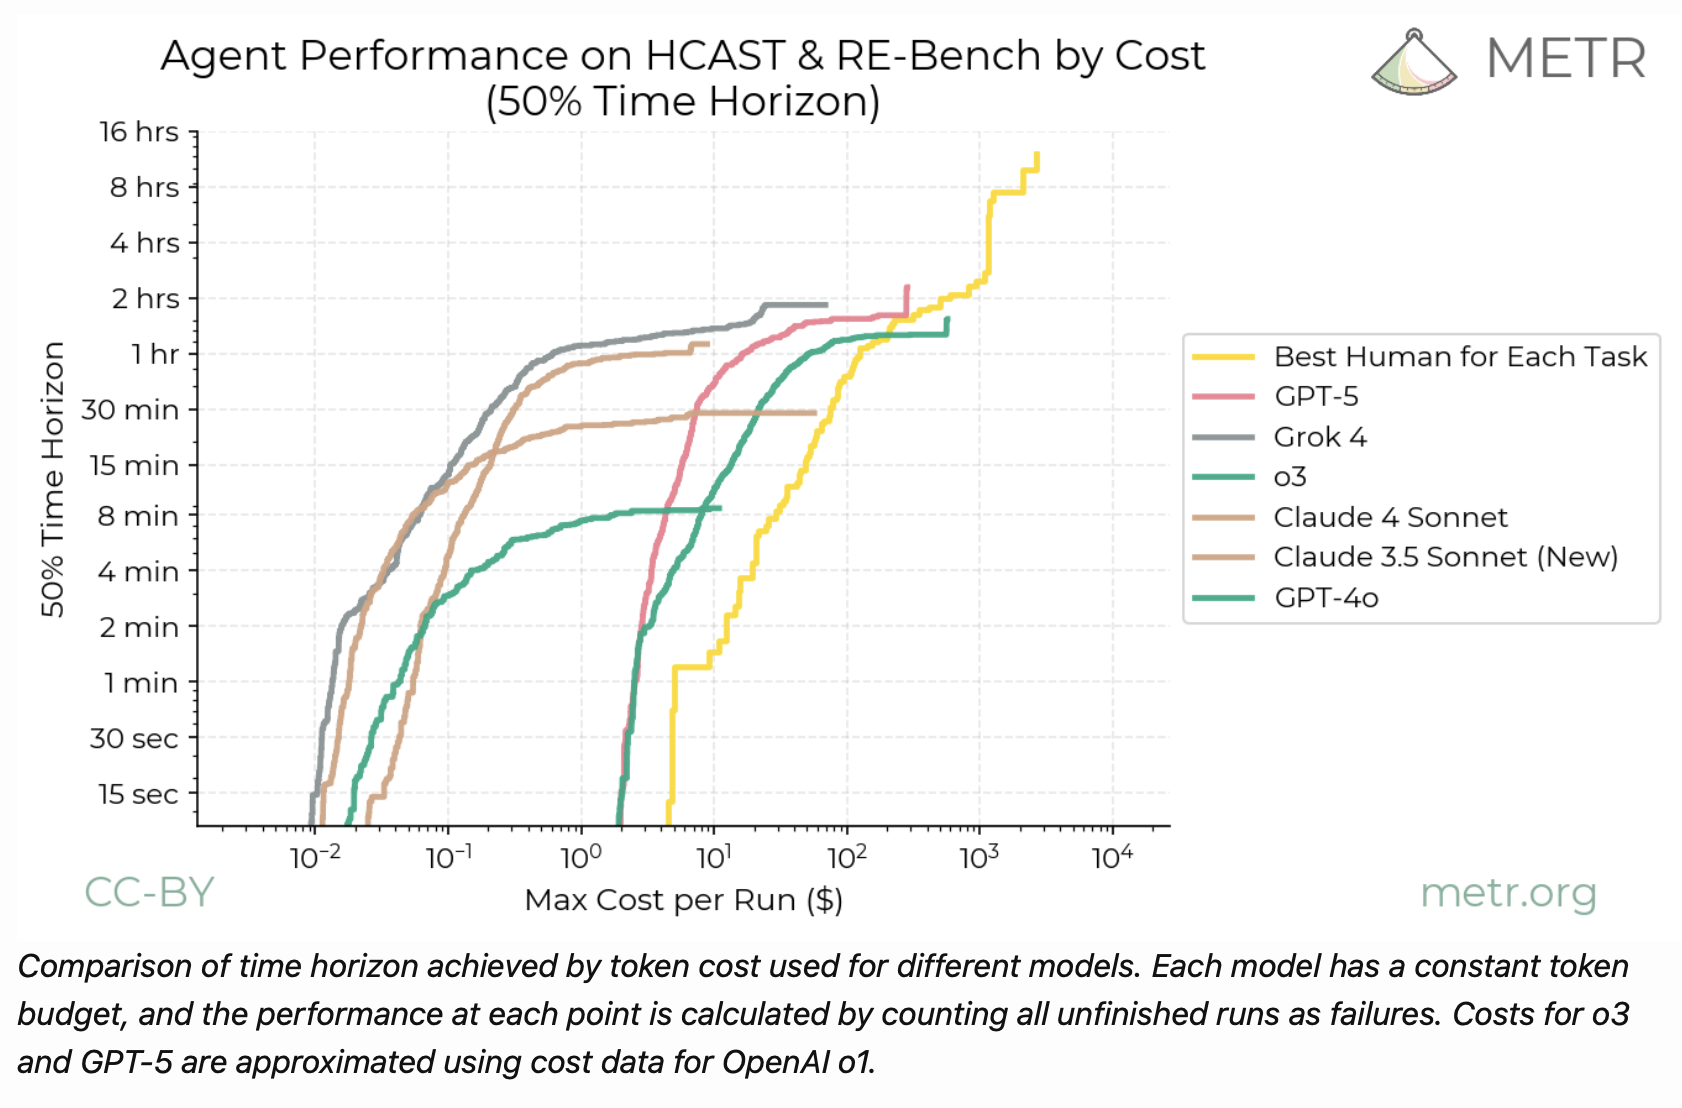
\includegraphics[keepaspectratio]{images/2025-09-19-16-04-34.png}}

}

\caption{Agent Performance on HCAST \& RE-Bench by Cost}

\end{figure}%

Exceptions:

\begin{itemize}
\tightlist
\item
  Computer transcription was for a period more accurate but less
  cost-effective than humans.
\item
  Reasoning tasks with high test-time expenditure
  (\href{https://arcprize.org/arc-agi}{ARC-AGI}))
\item
  \href{https://futuretech-site.s3.us-east-2.amazonaws.com/2024-01-18+Beyond_AI_Exposure.pdf}{Svanberg
  et al.~(2024)} argue that ``only 23\% of worker compensation
  ``exposed'' to AI computer vision would be cost-effective for firms to
  automate because of the large upfront costs of AI systems.'' However
  this is almost entirely fixed costs (data collection, fine tuning,
  scaffolding), not marginal costs.
\end{itemize}

\subsection{The economic impact of LLMs has been modest so
far}\label{the-economic-impact-of-llms-has-been-modest-so-far}

\begin{description}
\tightlist
\item[Around 1/2 of US adults regularly use an LLM-based chatbot.]
The productivity impact is perhaps 0.1-1\% of GDP:
\end{description}

\begin{itemize}
\tightlist
\item
  Bick, Blandin, and Deming (2024): 0.1-0.9\% aggregate productivity
  boost through time-savings on work tasks.
\item
  Humlum and Vestergaard (2025): 3\% average self-reported time saving
  among users.
\item
  Collis and Brynjolfsson (2025): genAI app users report valuations
  (Willingness-to-Accept) equivalent to around 0.3\% of GDP (\$98 per
  user, \$97B total).
\end{itemize}

\begin{description}
\tightlist
\item[Probably the biggest economic impact is on home production.]
Working on a paper documenting ChatGPT use. Note that Anthropic and
Microsoft papers only focus on use at work tasks.
\item[Enterprise impacts are still small.]
Most enterprises have adopted AI in some form, but they typically report
small effects on revenue or costs.
\end{description}

Maslej et al. (2025) say:

\begin{quote}
``Most companies that report financial impacts from using AI within a
business function estimate the benefits as being at low levels. 49\% of
respondents whose organizations use AI in service operations report cost
savings, followed by supply chain management (43\%) and software
engineering (41\%), but most of them report cost savings of less than
10\%.''
\end{quote}

\marginnote{\begin{footnotesize}

\pandocbounded{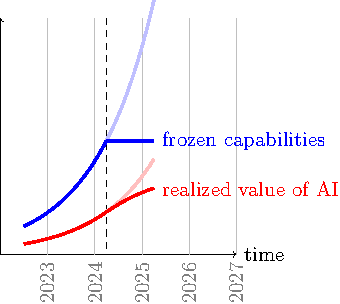
\includegraphics[keepaspectratio]{stylized-facts_files/figure-pdf/unnamed-chunk-4-1.pdf}}

\end{footnotesize}}

\textbf{Most growth in impact is likely due to capabilities rather than
diffusion.} Thought experiment: if we had frozen capabilities at
gpt-3.5, gpt-4.0, what would be the impact today?

We can observe the causal effect of model improvement on existing
cohorts with AB tests, it is harder to attribute user acquisition.

\subsection{We may not be able to direct technical
change}\label{we-may-not-be-able-to-direct-technical-change}

\textbf{Many economists have said we should shift the focus of our AI
research:}

Brynjolfsson (2023)

\begin{quote}
``an excessive focus on developing and deploying {[}human-level AI{]}
can lead us into a trap \ldots{} when AI is focused on augmenting humans
rather than mimicking them, then humans retain the power to insist on a
share of the value created''
\end{quote}

Acemoglu (2021):

\begin{quote}
``our current trajectory automates work to an excessive degree while
refusing to invest in human productivity
\end{quote}

\textbf{This may not be possible:} augmenting AI and automating AI may
be the same AI.

If there is a single latent factor of model ability, then work to train
an augmenting model looks very similar to work to train an automating
model. The ability to significantly steer AI capabilities seems limited.

\subsection{A univariate model of machine and human intelligence will be
a poor
fit}\label{a-univariate-model-of-machine-and-human-intelligence-will-be-a-poor-fit}

\begin{figure}[H]

{\centering \pandocbounded{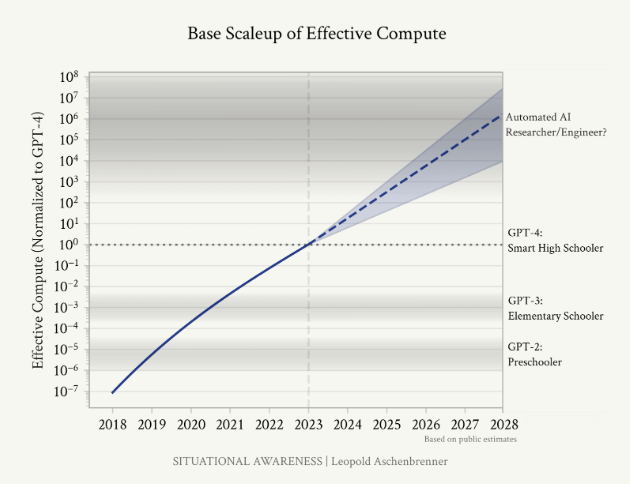
\includegraphics[keepaspectratio]{images/2025-07-17-07-40-28.png}}

}

\caption{from Aschenbrenner (2024)}

\end{figure}%

We sometimes describe AI capability by human equivalent, e.g.~years of
education (Aschenbrenner (2024)).

What would a two-factor model look like?

\begin{itemize}
\tightlist
\item
  LLMs have PhD-level knowledge and reasoning.
\item
  LLMs have preschool-level tactics.
\end{itemize}

\subsection{Wages are unlikely to be pinned down by the price of
compute}\label{wages-are-unlikely-to-be-pinned-down-by-the-price-of-compute}

Some models feature ``equilibrium task-sharing'': humans perform tasks
that computers are able to do, but it is too expensive for computers:

\begin{itemize}
\tightlist
\item
  Trammell and Korinek (2023)
\item
  Ide and Talamas (2024)
\item
  Noah Smith
  (\href{https://www.noahpinion.blog/p/plentiful-high-paying-jobs-in-the}{2024})
  on comparative advantage and wages.
\item
  Acemoglu (2024)
\item
  Jones (2025) assumes that all tasks which an AI can do will be done by
  an AI in equilibrium (assumption 1, p8). However he also expects that
  significant progress through a reduction in the price of AI tasks.
\end{itemize}

We argued above that equilibrium task-sharing has historically been true
only for a small share of tasks.

Equilibrium task-sharing would require either:

\begin{enumerate}
\def\labelenumi{\arabic{enumi}.}
\tightlist
\item
  A dramatic increase in the price to perform a task:

  \begin{itemize}
  \tightlist
  \item
    An increase in the compute required for new tasks -- the price of
    frontier inference has been steady.
  \item
    An increase in compute costs -- GPU rental prices have been steady,
    and the purchase/rent ratio has been stable.
  \item
    An increase in margins.
  \end{itemize}
\item
  A dramatic drop in human wages.
\end{enumerate}

\section{Appendix / Offcuts}\label{appendix-offcuts}

\href{https://www.jasonwei.net/blog/asymmetry-of-verification-and-verifiers-law}{Jason
Wei blog post} \emph{``The ease of training AI to solve a task is
proportional to how verifiable the task is. All tasks that are possible
to solve and easy to verify will be solved by AI''.} Five specific
factors:

\begin{enumerate}
\def\labelenumi{\arabic{enumi}.}
\tightlist
\item
  Objective truth: everyone agrees what good solutions are
\item
  Fast to verify: any given solution can be verified in a few seconds
\item
  Scalable to verify: many solutions can be verified simultaneously
\item
  Low noise: verification is as tightly correlated to the solution
  quality as possible
\item
  Continuous reward: it's easy to rank the goodness of many solutions
  for a single problem
\end{enumerate}

\section*{References}\label{references}
\addcontentsline{toc}{section}{References}

\phantomsection\label{refs}
\begin{CSLReferences}{1}{0}
\bibitem[\citeproctext]{ref-acemoglu2021ai}
Acemoglu, Daron. 2021. {``AI's Future Doesn't Have to Be Dystopian.''}
\emph{Boston Review} 20.

\bibitem[\citeproctext]{ref-acemoglu2024simple}
---------. 2024. {``The Simple Macroeconomics of AI.''} National Bureau
of Economic Research.

\bibitem[\citeproctext]{ref-agarwal2024radiology}
Agarwal, Nikhil, Alex Moehring, Pranav Rajpurkar, and Tobias Salz. 2024.
{``Combining Human Expertise with Artificial Intelligence: Experimental
Evidence from Radiology.''} MIT Department of Economics.
\url{https://economics.mit.edu/sites/default/files/inline-files/agarwal-et-al-diagnostic-ai\%20\%285\%29.pdf}.

\bibitem[\citeproctext]{ref-aschenbrenner2024situational}
Aschenbrenner, Leopold. 2024. {``Situational Awareness.''} \emph{The
Decade Ahead. Situational-Awareness. Ai}.

\bibitem[\citeproctext]{ref-backlund2025vending}
Backlund, Axel, and Lukas Petersson. 2025. {``Vending-Bench: A Benchmark
for Long-Term Coherence of Autonomous Agents.''} \emph{arXiv Preprint
arXiv:2502.15840}. \url{https://arxiv.org/abs/2502.15840}.

\bibitem[\citeproctext]{ref-bai2024longbench}
Bai, Yushi, Shangqing Tu, Jiajie Zhang, Hao Peng, Xiaozhi Wang, Xin Lv,
Shulin Cao, et al. 2024. {``LongBench V2: Towards Deeper Understanding
and Reasoning on Realistic Long-Context Multitasks.''} \emph{arXiv
Preprint arXiv:2412.15204}. \url{https://arxiv.org/abs/2412.15204}.

\bibitem[\citeproctext]{ref-balachandran2025inference}
Balachandran, Vidhisha, Jingya Chen, Lingjiao Chen, Shivam Garg, Neel
Joshi, Yash Lara, John Langford, et al. 2025. {``Inference-Time Scaling
for Complex Tasks: Where We Stand and What Lies Ahead.''} \emph{arXiv
Preprint arXiv:2504.00294}.

\bibitem[\citeproctext]{ref-becker2025developerproductivity}
Becker, Joel, Nate Rush, Beth Barnes, and David Rein. 2025. {``Measuring
the Impact of Early-2025 AI on Experienced Open-Source Developer
Productivity.''} \emph{arXiv Preprint arXiv:2507.09089}.
\url{https://arxiv.org/abs/2507.09089}.

\bibitem[\citeproctext]{ref-beeching2024scalingtesttimecompute}
Beeching, Edward, Lewis Tunstall, and Sasha Rush. 2024. {``Scaling
Test-Time Compute with Open Models.''}
\url{https://huggingface.co/spaces/HuggingFaceH4/blogpost-scaling-test-time-compute}.

\bibitem[\citeproctext]{ref-bick2024rapid}
Bick, Alexander, Adam Blandin, and David J Deming. 2024. {``The Rapid
Adoption of Generative AI.''} National Bureau of Economic Research.

\bibitem[\citeproctext]{ref-brynjolfsson2023turing}
Brynjolfsson, Erik. 2023. {``The Turing Trap: The Promise \& Peril of
Human-Like Artificial Intelligence.''} In \emph{Augmented Education in
the Global Age}, 103--16. Routledge.

\bibitem[\citeproctext]{ref-brynjolfsson2023callcenter}
Brynjolfsson, Erik, Danielle Li, and Lindsey R. Raymond. 2023.
{``Generative AI at Work.''} \emph{arXiv Preprint arXiv:2304.11771}.
\url{https://arxiv.org/abs/2304.11771}.

\bibitem[\citeproctext]{ref-burnell2023reveal}
Burnell, Richard, Heng Hao, Andrew R. A. Conway, and José
Hernández-Orallo. 2023. {``Revealing the Structure of Language Model
Capabilities.''} \emph{arXiv Preprint arXiv:2306.10062}.
\url{https://arxiv.org/abs/2306.10062}.

\bibitem[\citeproctext]{ref-choi2023legal}
Choi, Jonathan H., Amy Monahan, and Daniel Schwarcz. 2023. {``AI
Assistance in Legal Work: Evidence from a Field Experiment.''}
\emph{SSRN Electronic Journal}.
\url{https://doi.org/10.2139/ssrn.4626276}.

\bibitem[\citeproctext]{ref-chollet2019measureintelligence}
Chollet, François. 2019. {``On the Measure of Intelligence.''}
\url{https://arxiv.org/pdf/1911.01547.pdf}.

\bibitem[\citeproctext]{ref-choshen2024hitchhiker}
Choshen, Leshem, Yang Zhang, and Jacob Andreas. 2024. {``A Hitchhiker's
Guide to Scaling Law Estimation.''} \emph{arXiv Preprint
arXiv:2410.11840}.

\bibitem[\citeproctext]{ref-chui2023economic}
Chui, Michael, Eric Hazan, Roger Roberts, Alex Singla, and Kate Smaje.
2023. {``The Economic Potential of Generative AI.''}
\url{https://www.mckinsey.com/capabilities/mckinsey-digital/our-insights/the-economic-potential-of-generative-ai-the-next-productivity-frontier}.

\bibitem[\citeproctext]{ref-collis2025wta}
Collis, Avinash, and Erik Brynjolfsson. 2025. {``AI's Overlooked \$97
Billion Contribution to the Economy.''} \emph{The Wall Street Journal},
August.
\url{https://www.wsj.com/opinion/ais-overlooked-97-billion-contribution-to-the-economy-users-service-da6e8f55}.

\bibitem[\citeproctext]{ref-epoch2025llminferencepricetrends}
Cottier, Ben, Ben Snodin, David Owen, and Tom Adamczewski. 2025. {``LLM
Inference Prices Have Fallen Rapidly but Unequally Across Tasks.''}
\url{https://epoch.ai/data-insights/llm-inference-price-trends}.

\bibitem[\citeproctext]{ref-coupe2025impact}
Coupé, Tom, and Weilun Wu. 2025. {``The Impact of Generative AI on
Productivity: Results of an Early Meta-Analysis.''} 25/09. University of
Canterbury, Department of Economics; Finance.
\url{https://doi.org/None}.

\bibitem[\citeproctext]{ref-cui2024software}
Cui, Yiming, Mert Demirer, Sonia Jaffe, Andreas Musolff, Sida Peng, and
Tobias Salz. 2024. {``AI-Augmented Software Engineering: Evidence from a
Large-Scale Field Experiment.''} \emph{SSRN Electronic Journal}.
\url{https://doi.org/10.2139/ssrn.4945566}.

\bibitem[\citeproctext]{ref-dellacqua2023consultants}
Dell'Acqua, Fabrizio, Edward McFowland, Ethan R. Mollick, Hila
Lifshitz-Assaf, Katherine Kellogg, Saran Rajendran, Lisa Krayer,
François Candelon, and Karim R. Lakhani. 2023. {``Navigating the Jagged
Technological Frontier: Field Experimental Evidence of the Effects of AI
on Knowledge Worker Productivity and Quality.''} \emph{Harvard Business
School Working Paper}.
\url{https://www.hbs.edu/faculty/Pages/item.aspx?num=64700}.

\bibitem[\citeproctext]{ref-dorn2025temporal}
Dorn, Félix, Xavier Ferrés, Elsie Jang, and Valmik Nahata. 2025. {``The
Early Economic Impacts of Transformative AI: A Focus on Temporal
Coherence.''} Research submission for the „Economics of Transformative
AI'' initiative, organised by Apart Research.
\url{https://apartresearch.com/project/the-early-economic-impacts-of-transformative-ai-a-focus-on-temporal-coherence-ipql}.

\bibitem[\citeproctext]{ref-dreyfuss2025human}
Dreyfuss, Bnaya, and Raphaël Raux. 2025. {``Human Learning about AI:
Projection of Difficulty Distorts Beliefs.''} \emph{arXiv Preprint
arXiv:2406.05408}. \url{https://arxiv.org/abs/2406.05408}.

\bibitem[\citeproctext]{ref-eloundou2023gpts}
Eloundou, Tyna, Sam Manning, Pamela Mishkin, and Daniel Rock. 2023.
{``Gpts Are Gpts: An Early Look at the Labor Market Impact Potential of
Large Language Models.''} \emph{arXiv Preprint arXiv:2303.10130}.

\bibitem[\citeproctext]{ref-epoch2024optimallyallocating}
Erdil, Ege. 2024. {``Optimally Allocating Compute Between Inference and
Training.''}
\url{https://epoch.ai/blog/optimally-allocating-compute-between-inference-and-training}.

\bibitem[\citeproctext]{ref-gao2024github}
Gao, Albert. 2024. {``Research: Quantifying GitHub Copilot's Impact in
the Enterprise with Accenture.''}
\url{https://github.blog/2024-05-13-research-quantifying-github-copilots-impact-in-the-enterprise-with-accenture/\#from-the-lab-to-the-real-world}.

\bibitem[\citeproctext]{ref-google2025alphaevolve}
Google. 2025. {``AlphaEvolve: A Gemini-Powered Coding Agent for
Designing Advanced Algorithms.''}
\url{https://deepmind.google/discover/blog/alphaevolve-a-gemini-powered-coding-agent-for-designing-advanced-algorithms/}.

\bibitem[\citeproctext]{ref-haupt2025position}
Haupt, Andreas, and Erik Brynjolfsson. 2025. {``Position: {AI} Should
Not Be an Imitation Game: Centaur Evaluations.''} In \emph{Forty-Second
International Conference on Machine Learning Position Paper Track}.
\url{https://openreview.net/forum?id=LkdH35003E}.

\bibitem[\citeproctext]{ref-heitmann2025trajectories}
Heitmann, Max, Ture Hinrichsen, David Africa, and Jonas Sandbrink. 2025.
{``Understanding AI Trajectories: Mapping the Limitations of Current AI
Systems (24\_10 Update).''} AI Safety Institute.
\url{https://cdn.prod.website-files.com/663bd486c5e4c81588db7a1d/68fb86aa2c3b1b7ea6251cc1_Understanding\%20AI\%20Trajectories\%20(24_10\%20update).pdf}.

\bibitem[\citeproctext]{ref-hendrycks2025agidefinition}
Hendrycks, Dan, Dawn Song, Christian Szegedy, Honglak Lee, Yarin Gal,
Erik Brynjolfsson, Sharon Li, et al. 2025. {``A Definition of AGI:''}
\url{https://www.agidefinition.ai/paper.pdf}.

\bibitem[\citeproctext]{ref-hoffmann2022computeoptimal}
Hoffmann, Jordan, Sebastian Borgeaud, Arthur Mensch, et al. 2022.
{``Training Compute-Optimal Large Language Models.''} \emph{arXiv
Preprint arXiv:2203.15556}. \url{https://arxiv.org/abs/2203.15556}.

\bibitem[\citeproctext]{ref-hoffmann2025generative}
Hoffmann, Manuel, Sam Boysel, Frank Nagle, Sida Peng, and Kevin Xu.
2025. {``Generative AI and the Nature of Work.''} \emph{Harvard Business
School Strategy Unit Working Paper}, no. 25-021: 25--021.

\bibitem[\citeproctext]{ref-hu2025lmgamebench}
Hu, Lanxiang, Mingjia Huo, Yuxuan Zhang, Haoyang Yu, Eric P. Xing, Ion
Stoica, Tajana Rosing, Haojian Jin, and Hao Zhang. 2025.
{``Lmgame-Bench: How Good Are LLMs at Playing Games?''}
\url{https://arxiv.org/pdf/2505.15146.pdf}.

\bibitem[\citeproctext]{ref-huber2025llmsblooms}
Huber, Thomas, and Christina Niklaus. 2025. {``LLMs Meet Bloom's
Taxonomy: A Cognitive View on Large Language Model Evaluations.''} In
\emph{Proceedings of the 31st International Conference on Computational
Linguistics}, 5211--46. Abu Dhabi, UAE: Association for Computational
Linguistics. \url{https://aclanthology.org/2025.coling-main.350/}.

\bibitem[\citeproctext]{ref-humlum2025large}
Humlum, Anders, and Emilie Vestergaard. 2025. {``Large Language Models,
Small Labor Market Effects.''} National Bureau of Economic Research.

\bibitem[\citeproctext]{ref-ide2024artificialintelligenceknowledgeeconomy}
Ide, Enrique, and Eduard Talamas. 2024. {``Artificial Intelligence in
the Knowledge Economy.''} \url{https://arxiv.org/pdf/2312.05481.pdf}.

\bibitem[\citeproctext]{ref-ilic2024positive}
Ilić, David, and Gilles E. Gignac. 2024. {``Evidence of Interrelated
Cognitive-Like Capabilities in Large Language Models: Indications of
Artificial General Intelligence or Achievement?''} \emph{Intelligence}
106 (September): 101858.
\url{https://doi.org/10.1016/j.intell.2024.101858}.

\bibitem[\citeproctext]{ref-jones2025aiinrnd}
Jones, Benjamin F. 2025. {``Artificial Intelligence in Research and
Development.''} Working Paper w34312. National Bureau of Economic
Research. \url{https://doi.org/10.3386/w34312}.

\bibitem[\citeproctext]{ref-kadavath2022know}
Kadavath, Saurav, Tom Conerly, Amanda Askell, Tom Henighan, Dawn Drain,
Ethan Perez, Nicholas Schiefer, et al. 2022. {``Language Models (Mostly)
Know What They Know.''} \url{https://arxiv.org/pdf/2207.05221.pdf}.

\bibitem[\citeproctext]{ref-kaplan2020scalinglaws}
Kaplan, Jared, Sam McCandlish, Tom Henighan, Tom B. Brown, Benjamin
Chess, Rewon Child, Scott Gray, Alec Radford, Jeffrey Wu, and Dario
Amodei. 2020. {``Scaling Laws for Neural Language Models.''}
\url{https://arxiv.org/pdf/2001.08361.pdf}.

\bibitem[\citeproctext]{ref-kipnis2025metabench}
Kipnis, Alex, Konstantinos Voudouris, Luca M. Schulze Buschoff, and Eric
Schulz. 2025. {``Metabench - a Sparse Benchmark of Reasoning and
Knowledge in Large Language Models.''} In \emph{The Thirteenth
International Conference on Learning Representations}.
\url{https://openreview.net/forum?id=4T33izzFpK}.

\bibitem[\citeproctext]{ref-kwa2025longtasks}
Kwa, Timothy, Xia Liu, Yu Yuan, Tanish Singh, et al. 2025. {``Measuring
AI Ability to Complete Long Tasks.''} \emph{arXiv Preprint
arXiv:2503.14499}. \url{https://arxiv.org/abs/2503.14499}.

\bibitem[\citeproctext]{ref-lambdalabs_gpu_pricing}
Lambda Labs. 2025. {``Lambda Cloud GPU Pricing.''}
\url{https://lambdalabs.com/service/gpu-cloud/pricing}.

\bibitem[\citeproctext]{ref-legg2007definitions}
Legg, Shane, and Marcus Hutter. 2007a. {``A Collection of Definitions of
Intelligence.''} \emph{Frontiers in Artificial Intelligence and
Applications (Vol. 157)}, 17--24. \url{https://arxiv.org/abs/0706.3639}.

\bibitem[\citeproctext]{ref-legg2007universal}
---------. 2007b. {``Universal Intelligence: A Definition of Machine
Intelligence.''} \emph{Minds and Machines} 17 (4): 391--444.
\url{https://doi.org/10.1007/s11023-007-9079-x}.

\bibitem[\citeproctext]{ref-li2025perturbation}
Li, Xinyuan, Murong Xu, Wenbiao Tao, Hanlun Zhu, Yike Zhao, Jipeng
Zhang, and Yunshi Lan. 2025. {``RIDE: Difficulty Evolving Perturbation
with Item Response Theory for Mathematical Reasoning.''}
\url{https://arxiv.org/pdf/2511.04120.pdf}.

\bibitem[\citeproctext]{ref-maimon2025iq}
Maimon, Aviya, Amir DN Cohen, Gal Vishne, Shauli Ravfogel, and Reut
Tsarfaty. 2025. {``From Benchmarks to Skills: Low-Rank Factors for LLM
Evaluation.''} \url{https://arxiv.org/pdf/2507.20208.pdf}.

\bibitem[\citeproctext]{ref-maslej2025aiindex}
Maslej, Nestor, Loredana Fattorini, Raymond Perrault, Yolanda Gil,
Vanessa Parli, Njenga Kariuki, Emily Capstick, et al. 2025.
{``Artificial Intelligence Index Report 2025.''} \emph{arXiv Preprint
arXiv:2504.07139}.

\bibitem[\citeproctext]{ref-merali2024scaling}
Merali, Ali. 2024. {``Scaling Laws for Economic Productivity:
Experimental Evidence in LLM-Assisted Translation.''} \emph{arXiv
Preprint arXiv:2409.02391}. \url{https://arxiv.org/abs/2409.02391}.

\bibitem[\citeproctext]{ref-metr2024capability}
METR. 2024. {``An Update on Our General Capability Evaluations.''}
\url{https://metr.org/blog/2024-08-06-update-on-evaluations/}.

\bibitem[\citeproctext]{ref-metr2025gpt5evaluation}
---------. 2025. {``Details about METR's Evaluation of OpenAI GPT-5.''}
\url{https://evaluations.metr.org/gpt-5-report/}.

\bibitem[\citeproctext]{ref-min2023factscore}
Min, Sewon, Kalpesh Krishna, Xinxi Lyu, et al. 2023. {``FActScore:
Fine-Grained Atomic Evaluation of Factual Precision in Long Form Text
Generation.''} \emph{arXiv Preprint arXiv:2305.14251}.
\url{https://arxiv.org/abs/2305.14251}.

\bibitem[\citeproctext]{ref-mirzadeh2024gsm}
Mirzadeh, Iman, Keivan Alizadeh, Hooman Shahrokhi, Oncel Tuzel, Samy
Bengio, and Mehrdad Farajtabar. 2024. {``GSM-Symbolic: Understanding the
Limitations of Mathematical Reasoning in Large Language Models.''}
\emph{arXiv Preprint arXiv:2410.05229}.
\url{https://arxiv.org/abs/2410.05229}.

\bibitem[\citeproctext]{ref-miserendino2025swelancer}
Miserendino, Samuel, Michele Wang, Tejal Patwardhan, and Johannes
Heidecke. 2025. {``SWE-Lancer: Can Frontier LLMs Earn \$1 Million from
Real-World Freelance Software Engineering?''}
\url{https://arxiv.org/pdf/2502.12115.pdf}.

\bibitem[\citeproctext]{ref-morris2023levels}
Morris, Meredith Ringel, Jascha Sohl-Dickstein, Noah Fiedel, Tris
Warkentin, Allan Dafoe, Aleksandra Faust, Clement Farabet, and Shane
Legg. 2023. {``Levels of AGI for Operationalizing Progress on the Path
to AGI.''} \emph{arXiv Preprint arXiv:2311.02462}.

\bibitem[\citeproctext]{ref-noy2023writing}
Noy, Shakked, and Whitney Zhang. 2023. {``Experimental Evidence on the
Productivity Effects of Generative Artificial Intelligence.''}
\emph{Science} 381 (6654): 187--92.
\url{https://doi.org/10.1126/science.adh2586}.

\bibitem[\citeproctext]{ref-oecd2025aicapabilityindicatorsfullreport}
OECD. 2025. {``Introducing the OECD AI Capability Indicators.''} Paris:
OECD Publishing. \url{https://doi.org/10.1787/be745f04-en}.

\bibitem[\citeproctext]{ref-openai2024simpleqa}
OpenAI. 2024. {``Introducing SimpleQA.''}
\url{https://openai.com/index/introducing-simpleqa/}.

\bibitem[\citeproctext]{ref-ord2025halflife}
Ord, Toby. 2025. {``The Half-Life of AI Success: A Model of Performance
Decay.''} \url{https://www.tobyord.com/writing/half-life}.

\bibitem[\citeproctext]{ref-otis2024entrepreneurs}
Otis, Christopher et al. 2024. {``AI-Augmented Entrepreneurship:
Evidence from a Field Experiment.''} \emph{SSRN Electronic Journal}.
\url{https://doi.org/10.2139/ssrn.4671369}.

\bibitem[\citeproctext]{ref-owen2024predictable}
Owen, David. 2024. {``How Predictable Is Language-Model Benchmark
Performance?''} \emph{arXiv Preprint arXiv:2401.04757}.
\url{https://arxiv.org/abs/2401.04757}.

\bibitem[\citeproctext]{ref-payne2025strategic}
Payne, Kenneth, and Baptiste Alloui-Cros. 2025. {``Strategic
Intelligence in Large Language Models: Evidence from Evolutionary Game
Theory.''} \emph{arXiv Preprint arXiv:2507.02618}.
\url{https://arxiv.org/abs/2507.02618}.

\bibitem[\citeproctext]{ref-peng2023developerproductivity}
Peng, Sida, Eirini Kalliamvakou, Peter Cihon, and Mert Demirer. 2023.
{``The Impact of AI on Developer Productivity: Evidence from GitHub
Copilot.''} \url{https://arxiv.org/pdf/2302.06590.pdf}.

\bibitem[\citeproctext]{ref-phan2025textquests}
Phan, Long, Mantas Mazeika, Andy Zou, and Dan Hendrycks. 2025.
{``TextQuests: How Good Are LLMs at Text-Based Video Games?''}
\emph{arXiv Preprint arXiv:2507.23701}.
\url{https://arxiv.org/abs/2507.23701}.

\bibitem[\citeproctext]{ref-polo2025sloth}
Polo, Felipe Maia, Seamus Somerstep, Leshem Choshen, Yuekai Sun, and
Mikhail Yurochkin. 2025. {``Sloth: Scaling Laws for LLM Skills to
Predict Multi-Benchmark Performance Across Families.''}
\url{https://arxiv.org/pdf/2412.06540.pdf}.

\bibitem[\citeproctext]{ref-renze2024effect}
Renze, Matthew, and Erhan Guven. 2024. {``The Effect of Sampling
Temperature on Problem Solving in Large Language Models.''} \emph{arXiv
Preprint arXiv:2402.05201}. \url{https://arxiv.org/abs/2402.05201}.

\bibitem[\citeproctext]{ref-ruan2024observational}
Ruan, Yizhong, Chris J. Maddison, and Tatsunori B. Hashimoto. 2024.
{``Observational Scaling Laws and the Predictability of Language-Model
Performance.''} \emph{arXiv Preprint arXiv:2405.10938}.
\url{https://arxiv.org/abs/2405.10938}.

\bibitem[\citeproctext]{ref-song2024good}
Song, Yifan, Guoyin Wang, Sujian Li, and Bill Yuchen Lin. 2024. {``The
Good, the Bad, and the Greedy: Evaluation of LLMs Should Not Ignore
Non-Determinism.''} \emph{arXiv Preprint arXiv:2407.10457}.
\url{https://arxiv.org/abs/2407.10457}.

\bibitem[\citeproctext]{ref-spangher2024generalized}
Spangher, Lewis, Tao Li, William F. Arnold, et al. 2024. {``Towards a
Generalized Performance Benchmark for LLM Capabilities.''} \emph{arXiv
Preprint arXiv:2410.22368}. \url{https://arxiv.org/abs/2410.22368}.

\bibitem[\citeproctext]{ref-sutton2019bitter}
Sutton, Richard. 2019. {``The Bitter Lesson.''} \emph{Incomplete Ideas
(Blog)} 13 (1): 38.
\url{http://www.incompleteideas.net/IncIdeas/BitterLesson.html}.

\bibitem[\citeproctext]{ref-toner2025takingjaggedness}
Toner, Helen. 2025. {``Taking Jaggedness Seriously.''} Substack ---
Rising Tide.

\bibitem[\citeproctext]{ref-trammell2023economic}
Trammell, Philip, and Anton Korinek. 2023. {``Economic Growth Under
Transformative AI.''} National Bureau of Economic Research.

\bibitem[\citeproctext]{ref-vaccaro2024humanai}
Vaccaro, Michelle, Abdullah Almaatouq, and Thomas Malone. 2024. {``When
Combinations of Humans and AI Are Useful: A Systematic Review and
Meta-Analysis.''} \emph{Nature Human Behaviour} 8: 2293--303.
\url{https://doi.org/10.1038/s41562-024-02024-1}.

\bibitem[\citeproctext]{ref-vafa2024worldmodel}
Vafa, Keyon, Justin Y. Chen, Ashesh Rambachan, Jon Kleinberg, and
Sendhil Mullainathan. 2024. {``Evaluating the World Model Implicit in a
Generative Model.''} In \emph{Advances in Neural Information Processing
Systems}, edited by A. Globerson, L. Mackey, D. Belgrave, A. Fan, U.
Paquet, J. Tomczak, and C. Zhang, 37:26941--75. Curran Associates, Inc.
\url{https://proceedings.neurips.cc/paper_files/paper/2024/file/2f6a6317bada76b26a4f61bb70a7db59-Paper-Conference.pdf}.

\bibitem[\citeproctext]{ref-vafa2024humangeneralization}
Vafa, Keyon, Ashesh Rambachan, and Sendhil Mullainathan. 2024. {``Do
Large Language Models Perform the Way People Expect? Measuring the Human
Generalization Function.''} \emph{arXiv Preprint arXiv:2406.01382}.
\url{https://arxiv.org/abs/2406.01382}.

\bibitem[\citeproctext]{ref-valmeekam2024llms}
Valmeekam, Karthik, Kaya Stechly, and Subbarao Kambhampati. 2024.
{``LLMs Still Can't Plan; Can LRMs? A Preliminary Evaluation of OpenAI's
O1 on PlanBench.''} \emph{arXiv Preprint arXiv:2409.13373}.
\url{https://arxiv.org/abs/2409.13373}.

\bibitem[\citeproctext]{ref-wang2023selfconsistency}
Wang, Xuezhi, Jason Wei, Dale Schuurmans, Quoc Le, Ed Chi, Sharan
Narang, Aakanksha Chowdhery, and Denny Zhou. 2023. {``Self-Consistency
Improves Chain of Thought Reasoning in Language Models.''}
\url{https://arxiv.org/pdf/2203.11171.pdf}.

\bibitem[\citeproctext]{ref-wei2024longformfactuality}
Wei, Jerry, Chengrun Yang, Xinying Song, et al. 2024. {``Long-Form
Factuality in Large Language Models.''} \emph{arXiv Preprint
arXiv:2403.18802}. \url{https://arxiv.org/abs/2403.18802}.

\bibitem[\citeproctext]{ref-vonwerra2025jaggeddata}
Werra, Leandro von. 2025. {``The Jagged AI Frontier Is a Data
Frontier.''} 2025.
\url{https://huggingface.co/spaces/lvwerra/jagged-data-frontier}.

\bibitem[\citeproctext]{ref-wu2025inferencescaling}
Wu, Yangzhen, Zhiqing Sun, Shanda Li, Sean Welleck, and Yiming Yang.
2025. {``Inference Scaling Laws: An Empirical Analysis of
Compute-Optimal Inference for Problem-Solving with Language Models.''}
\url{https://arxiv.org/pdf/2408.00724.pdf}.

\bibitem[\citeproctext]{ref-epoch2025howfarcanreasoningmodelsscale}
You, Josh. 2025. {``How Far Can Reasoning Models Scale?''}
\url{https://epoch.ai/gradient-updates/how-far-can-reasoning-models-scale}.

\bibitem[\citeproctext]{ref-zhang2025trainbeforetest}
Zhang, Guanhua, Ricardo Dominguez-Olmedo, and Moritz Hardt. 2025.
{``Train-Before-Test Harmonizes Language Model Rankings.''}
\url{https://doi.org/10.48550/arXiv.2507.05195}.

\bibitem[\citeproctext]{ref-zhou2025generalscales}
Zhou, Lexin, Lorenzo Pacchiardi, Fernando Martínez-Plumed, Katherine M.
Collins, Yael Moros-Daval, Seraphina Zhang, Qinlin Zhao, et al. 2025.
{``General Scales Unlock AI Evaluation with Explanatory and Predictive
Power.''} \url{https://arxiv.org/pdf/2503.06378.pdf}.

\bibitem[\citeproctext]{ref-zhou2024reliable}
Zhou, Lucy, Winfried Schellaert, Fernando Martínez-Plumed, et al. 2024.
{``Larger and More Instructable Language Models Become Less Reliable.''}
\emph{Nature} 634: 61--69.
\url{https://doi.org/10.1038/s41586-024-07930-y}.

\end{CSLReferences}




\end{document}
